\chapter{Application Mock-up}
\label{chapter:mockups}

% ==============================================================================
%                              USER VIEWS SECTION 
% ==============================================================================
\section{User Views}
\subsection{Registration and Login}
To be able to use the services of \textit{Room.io}, a User needs to be logged into their account by entering an email and password. If they have not yet registered on the system, a registration as either a Host or a Guest is necessary. To sign up, they simply need to enter: first and last name, email, password, and their Role. After submitting this information, the User receives an email to confirm the details which they need to respond to in order to become a Verified User. An Admin can only be added by an existing Admin as described in section \ref{admindashboard_section}.
 
\begin{figure}[H]
  \centering
  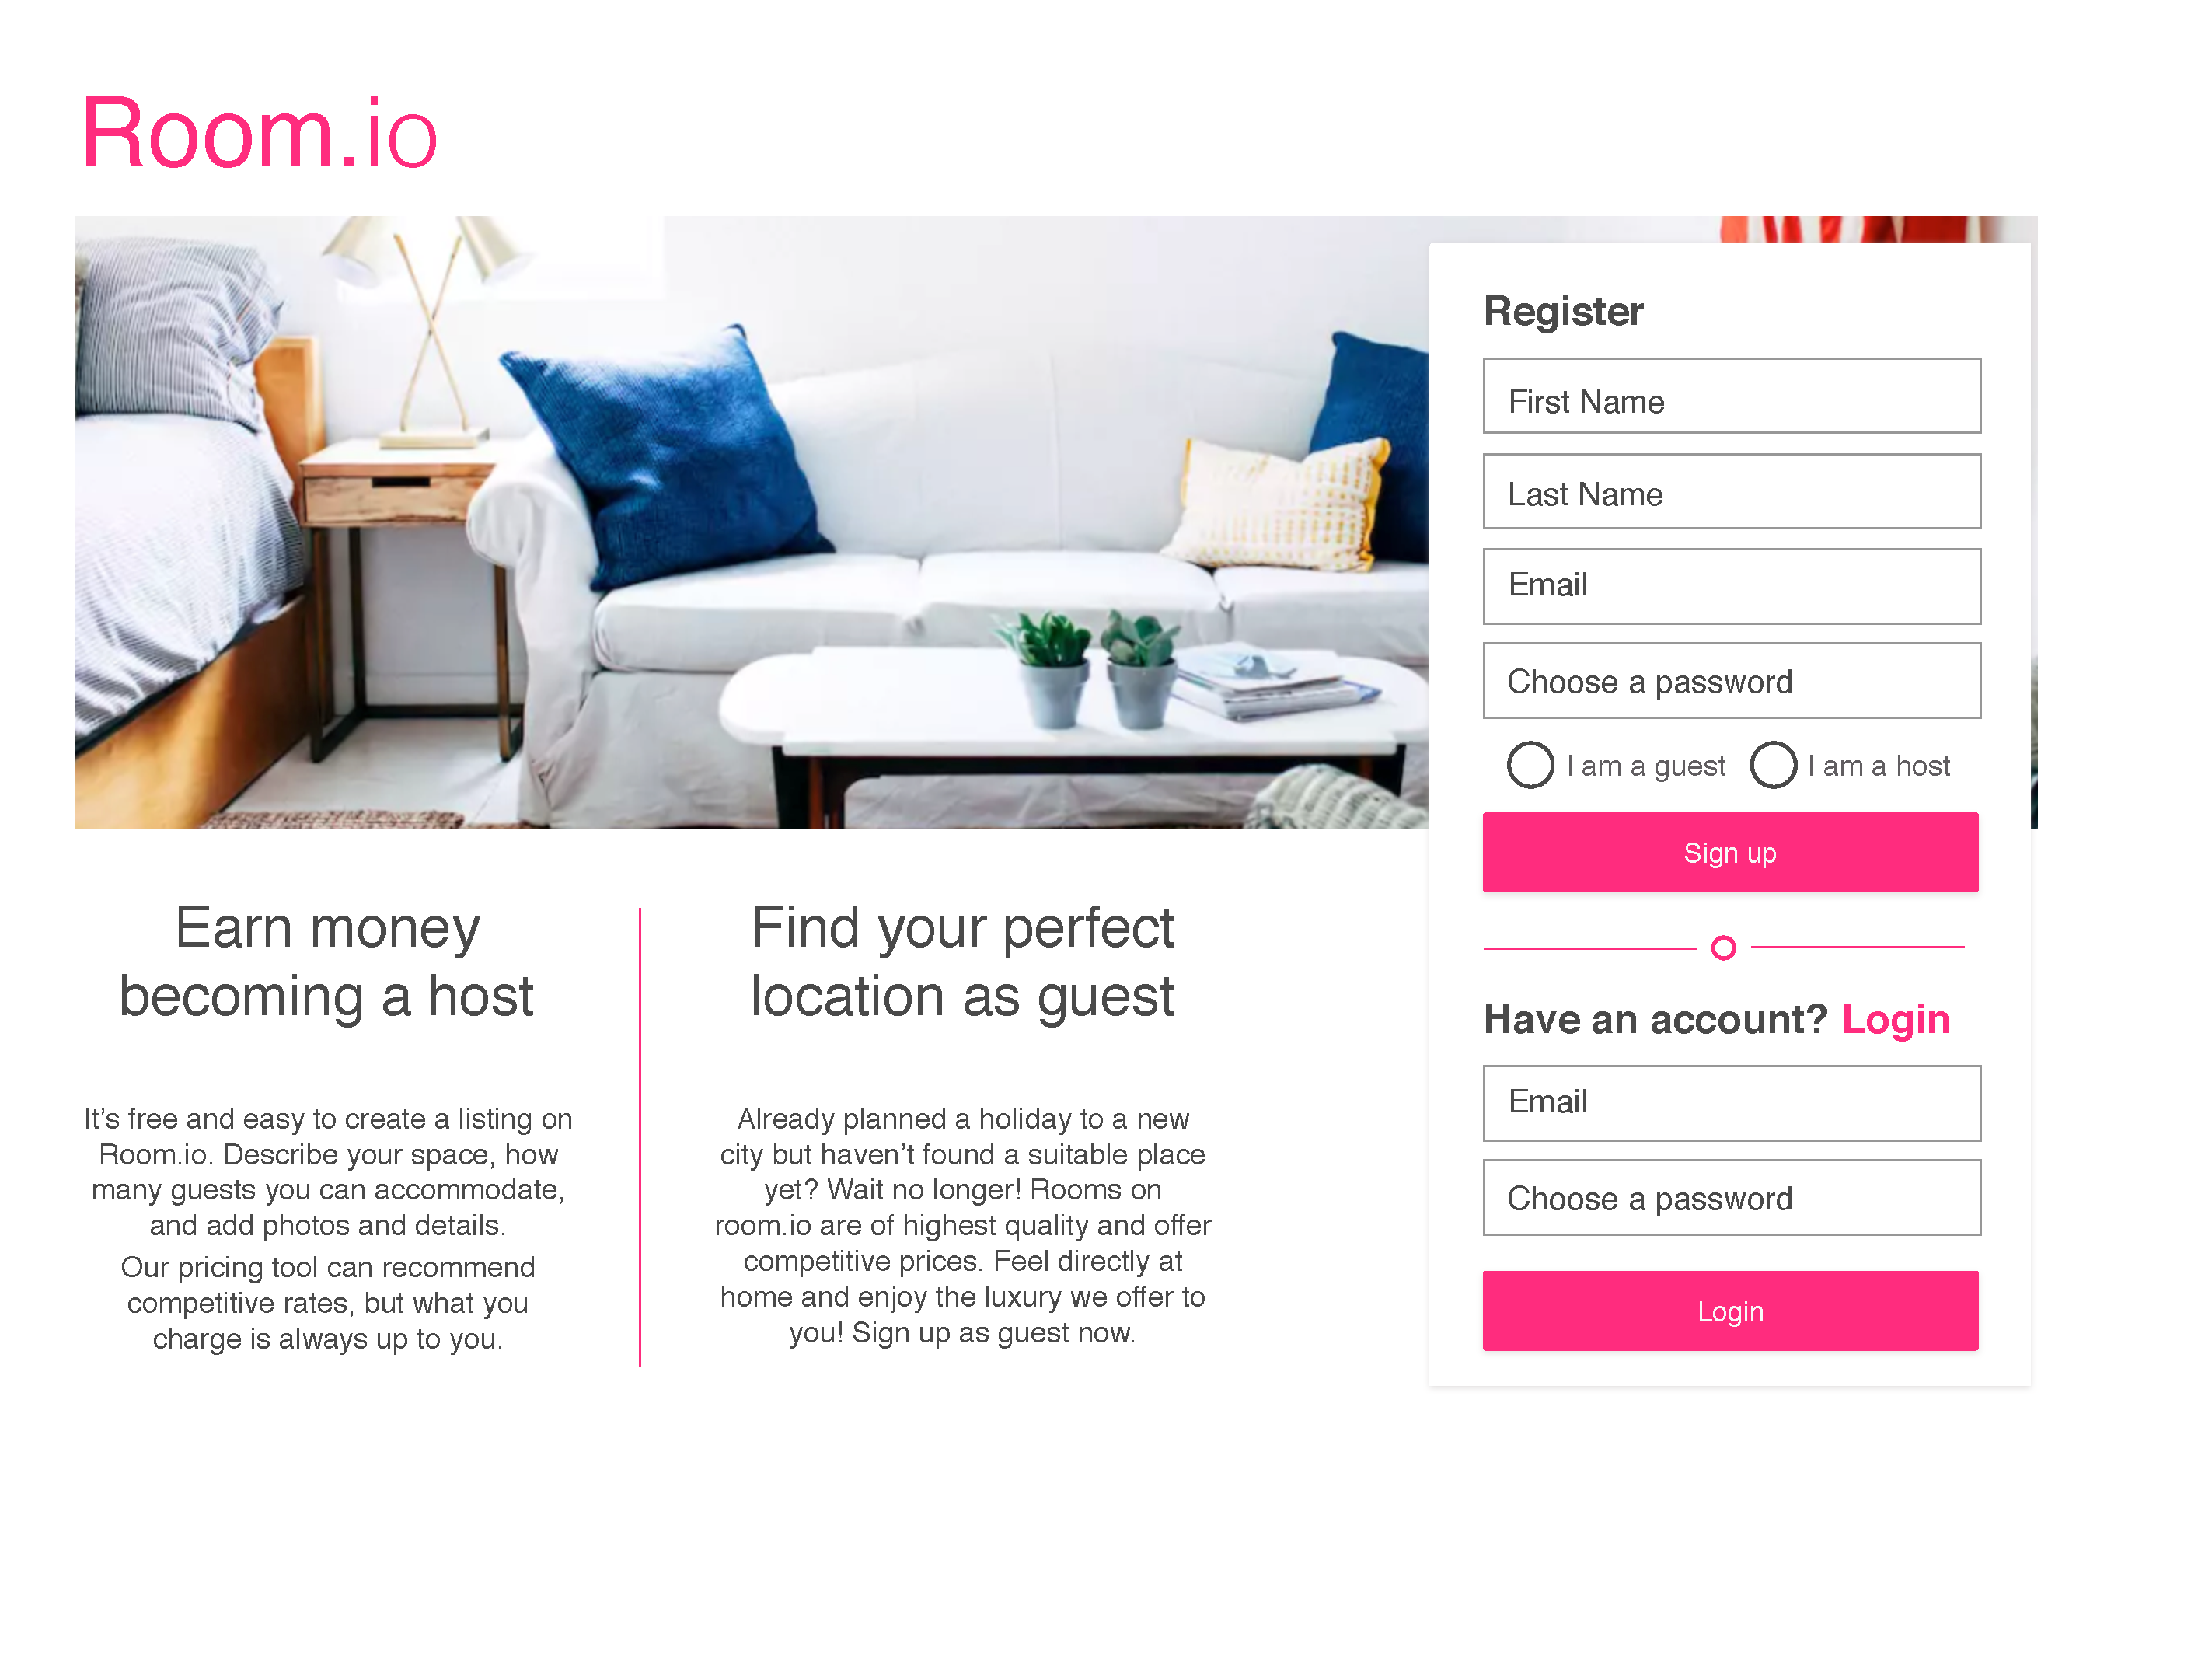
\includegraphics[width=17cm]{img/mockups/user_registration.pdf}
  \caption{Registration and Login View}
  \label{Registration_Login_View}
\end{figure}

\subsection{Profile Page}
To view and edit one's personal details, the Guest/Host can visit their profile page from the search page. Here they can update their information such as first and last name, email, and password.

\begin{figure}[H]
  \centering
  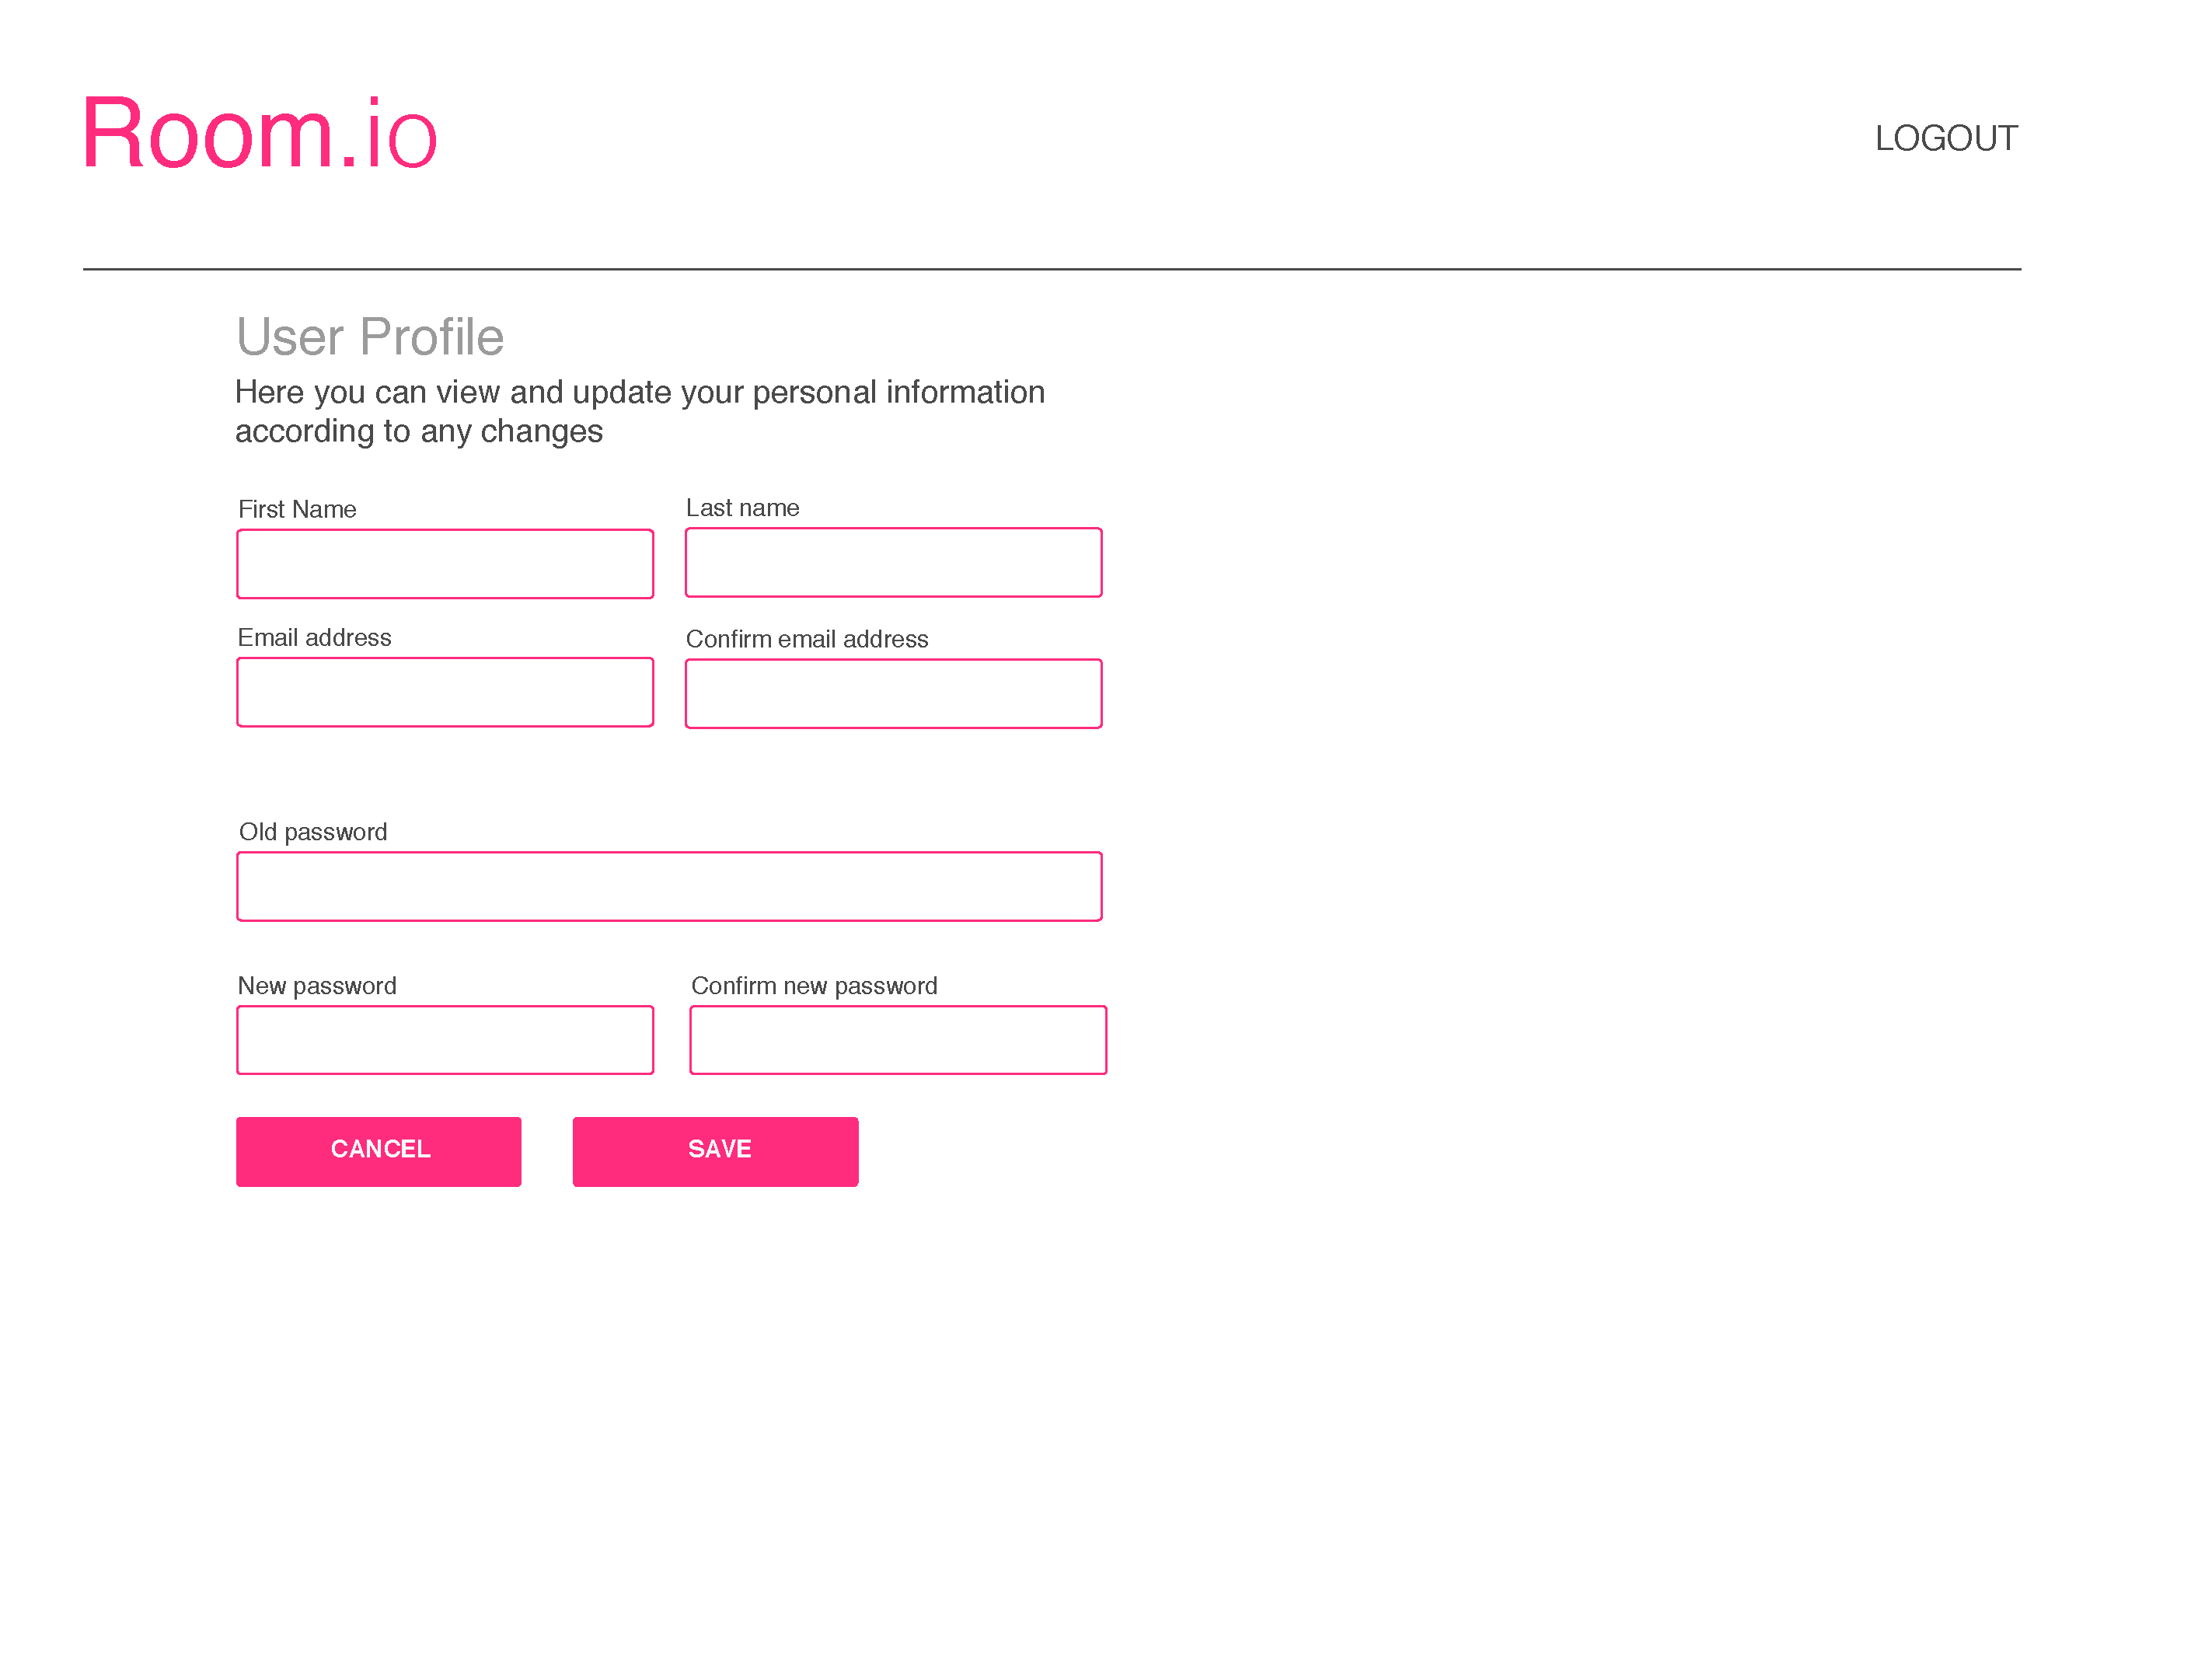
\includegraphics[width=17cm]{img/mockups/user_profile.pdf}
  \caption{Profile page}
  \label{Profile_View}
\end{figure}

% ==============================================================================
%                              GUEST VIEWS SECTION 
% ==============================================================================
\section{Guest Views}
\subsection{Search Request}
This is the page the Guest lands on after logging onto the system. Here they can search for a destination and have the option to indicate a time period for their stay, the number of people travelling as well as the number of rooms needed. Only the choice of a destination is mandatory; the other information can be edited on the detailed property view. The Guest can always return from any other page to this one by clicking on the \textit{Room.io} logo.

\begin{figure}[H]
  \centering
  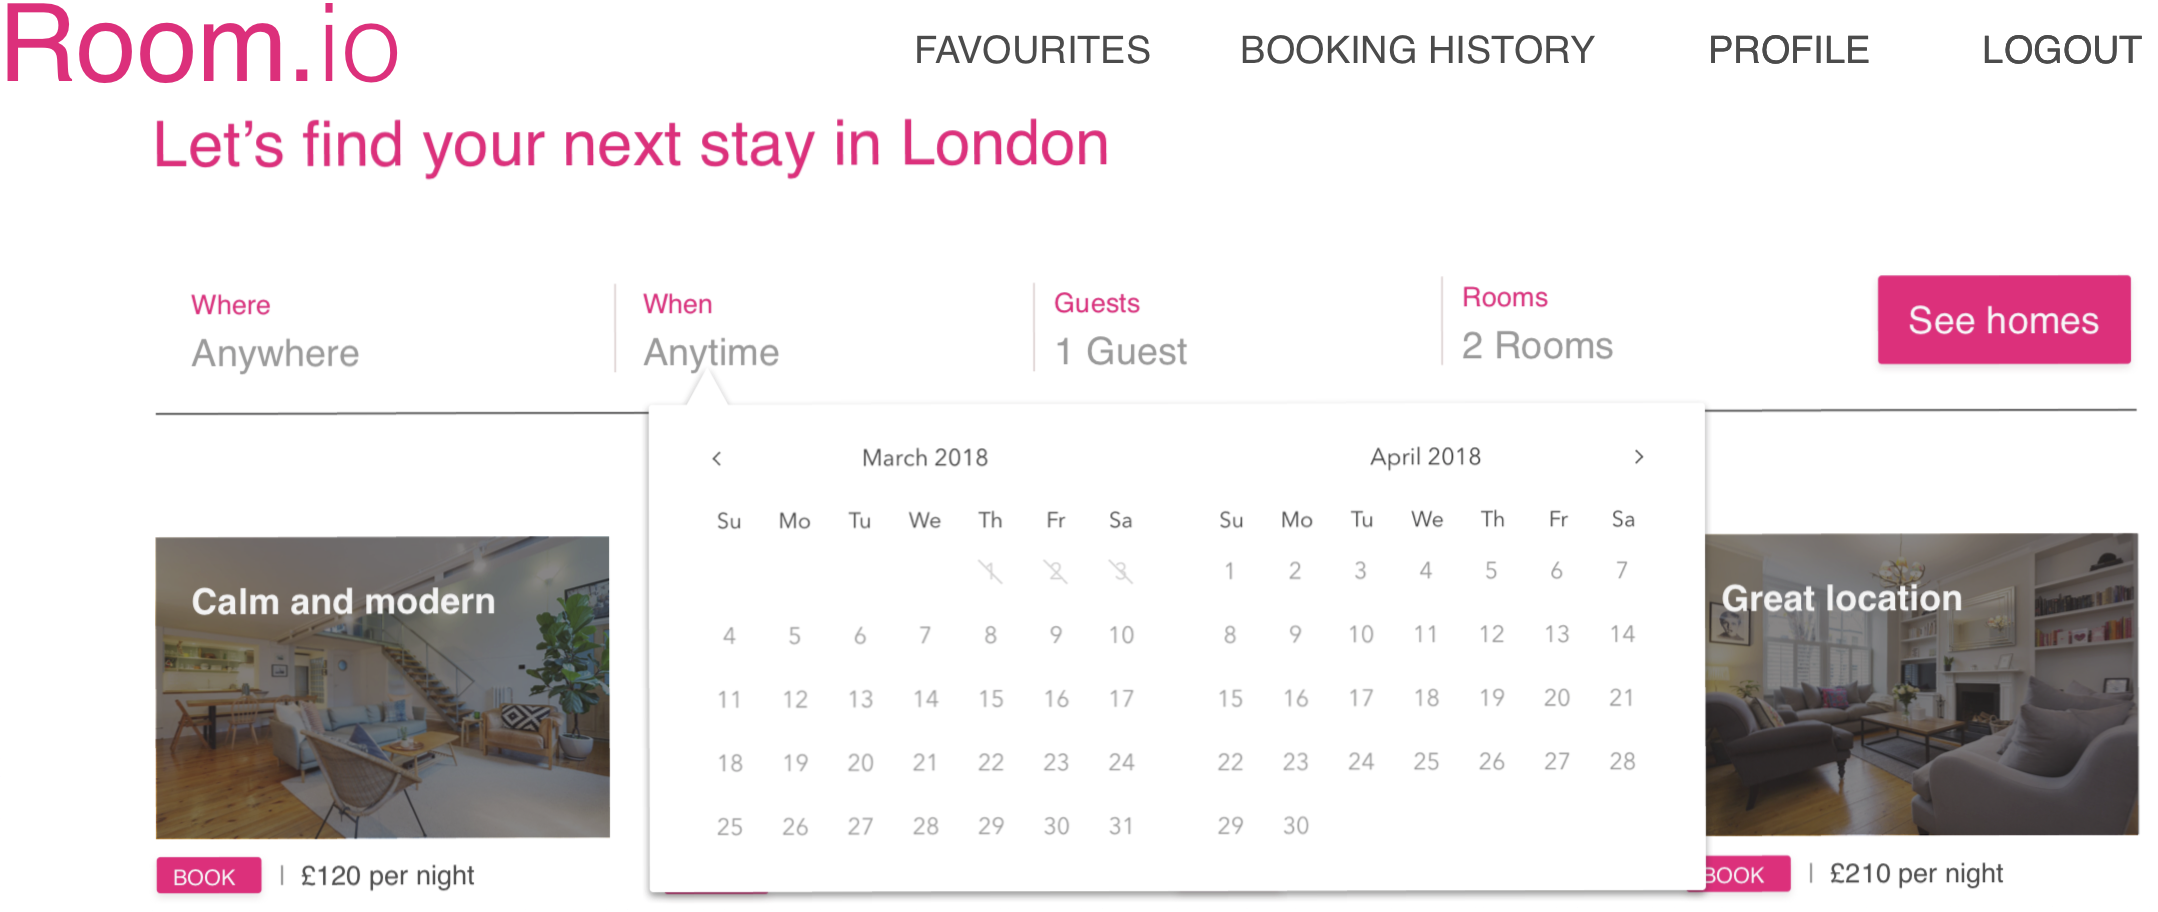
\includegraphics[width=\textwidth]{img/mockups/guest_search.png}
  \caption{Making a search request}
  \label{Search_View}
\end{figure}

\subsection{Property List View}
After sending a search request, the Guest sees a map of the chosen city with tags showing the price per night at the location of a property adhering to the chosen requirements. Underneath the map, a list of these properties is shown. By hovering over a tag, the respective location is highlighted in the list. The Guest also has the option to filter this list by the number of available rooms, room policies and ratings.

\begin{figure}[H]
  \centering
  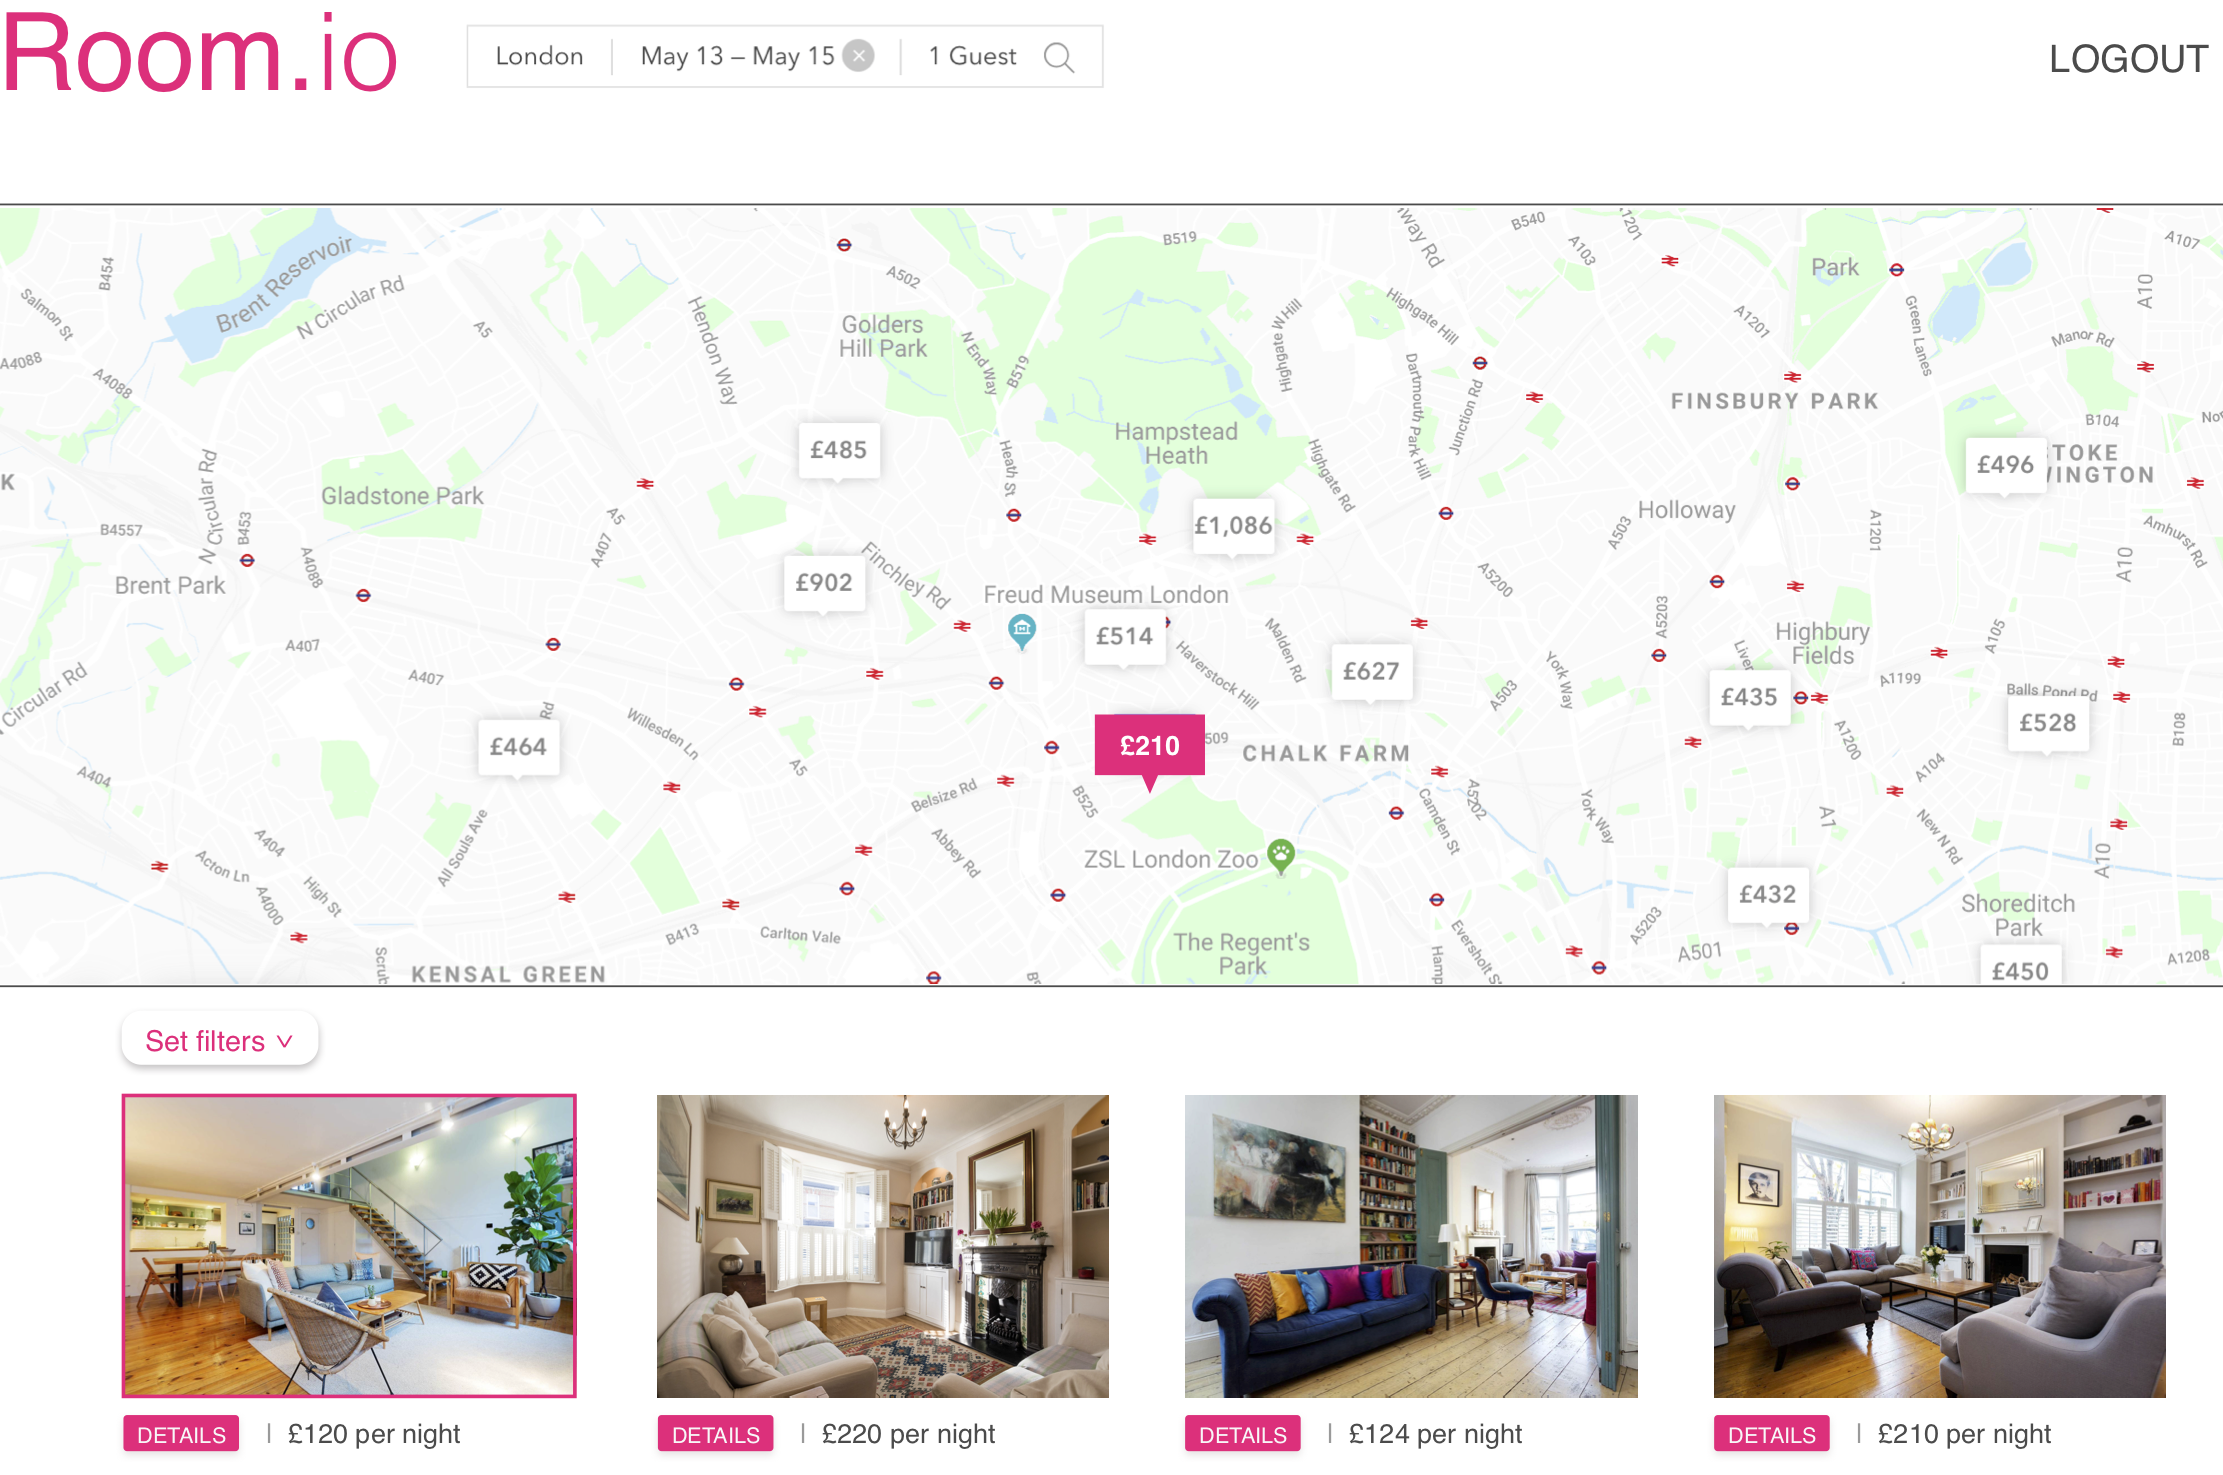
\includegraphics[width=17cm]{img/mockups/guest_propertyList.png}
  \caption{Property list view}
  \label{Property_List_View}
\end{figure}

\subsection{Detailed Property View}
After selecting a property, the Guest is able to see property pictures in a carousel as well as a detailed property description. Furthermore, the property's available rooms with a short description and policy attributes are depicted. When hovering over the star rating, a list of all given ratings for this room appears. The Guest is able to check the room's availability for a certain date and make a booking for a room. Additionally, they can add the property to their "favourites" list.

\begin{figure}[H]
  \centering
  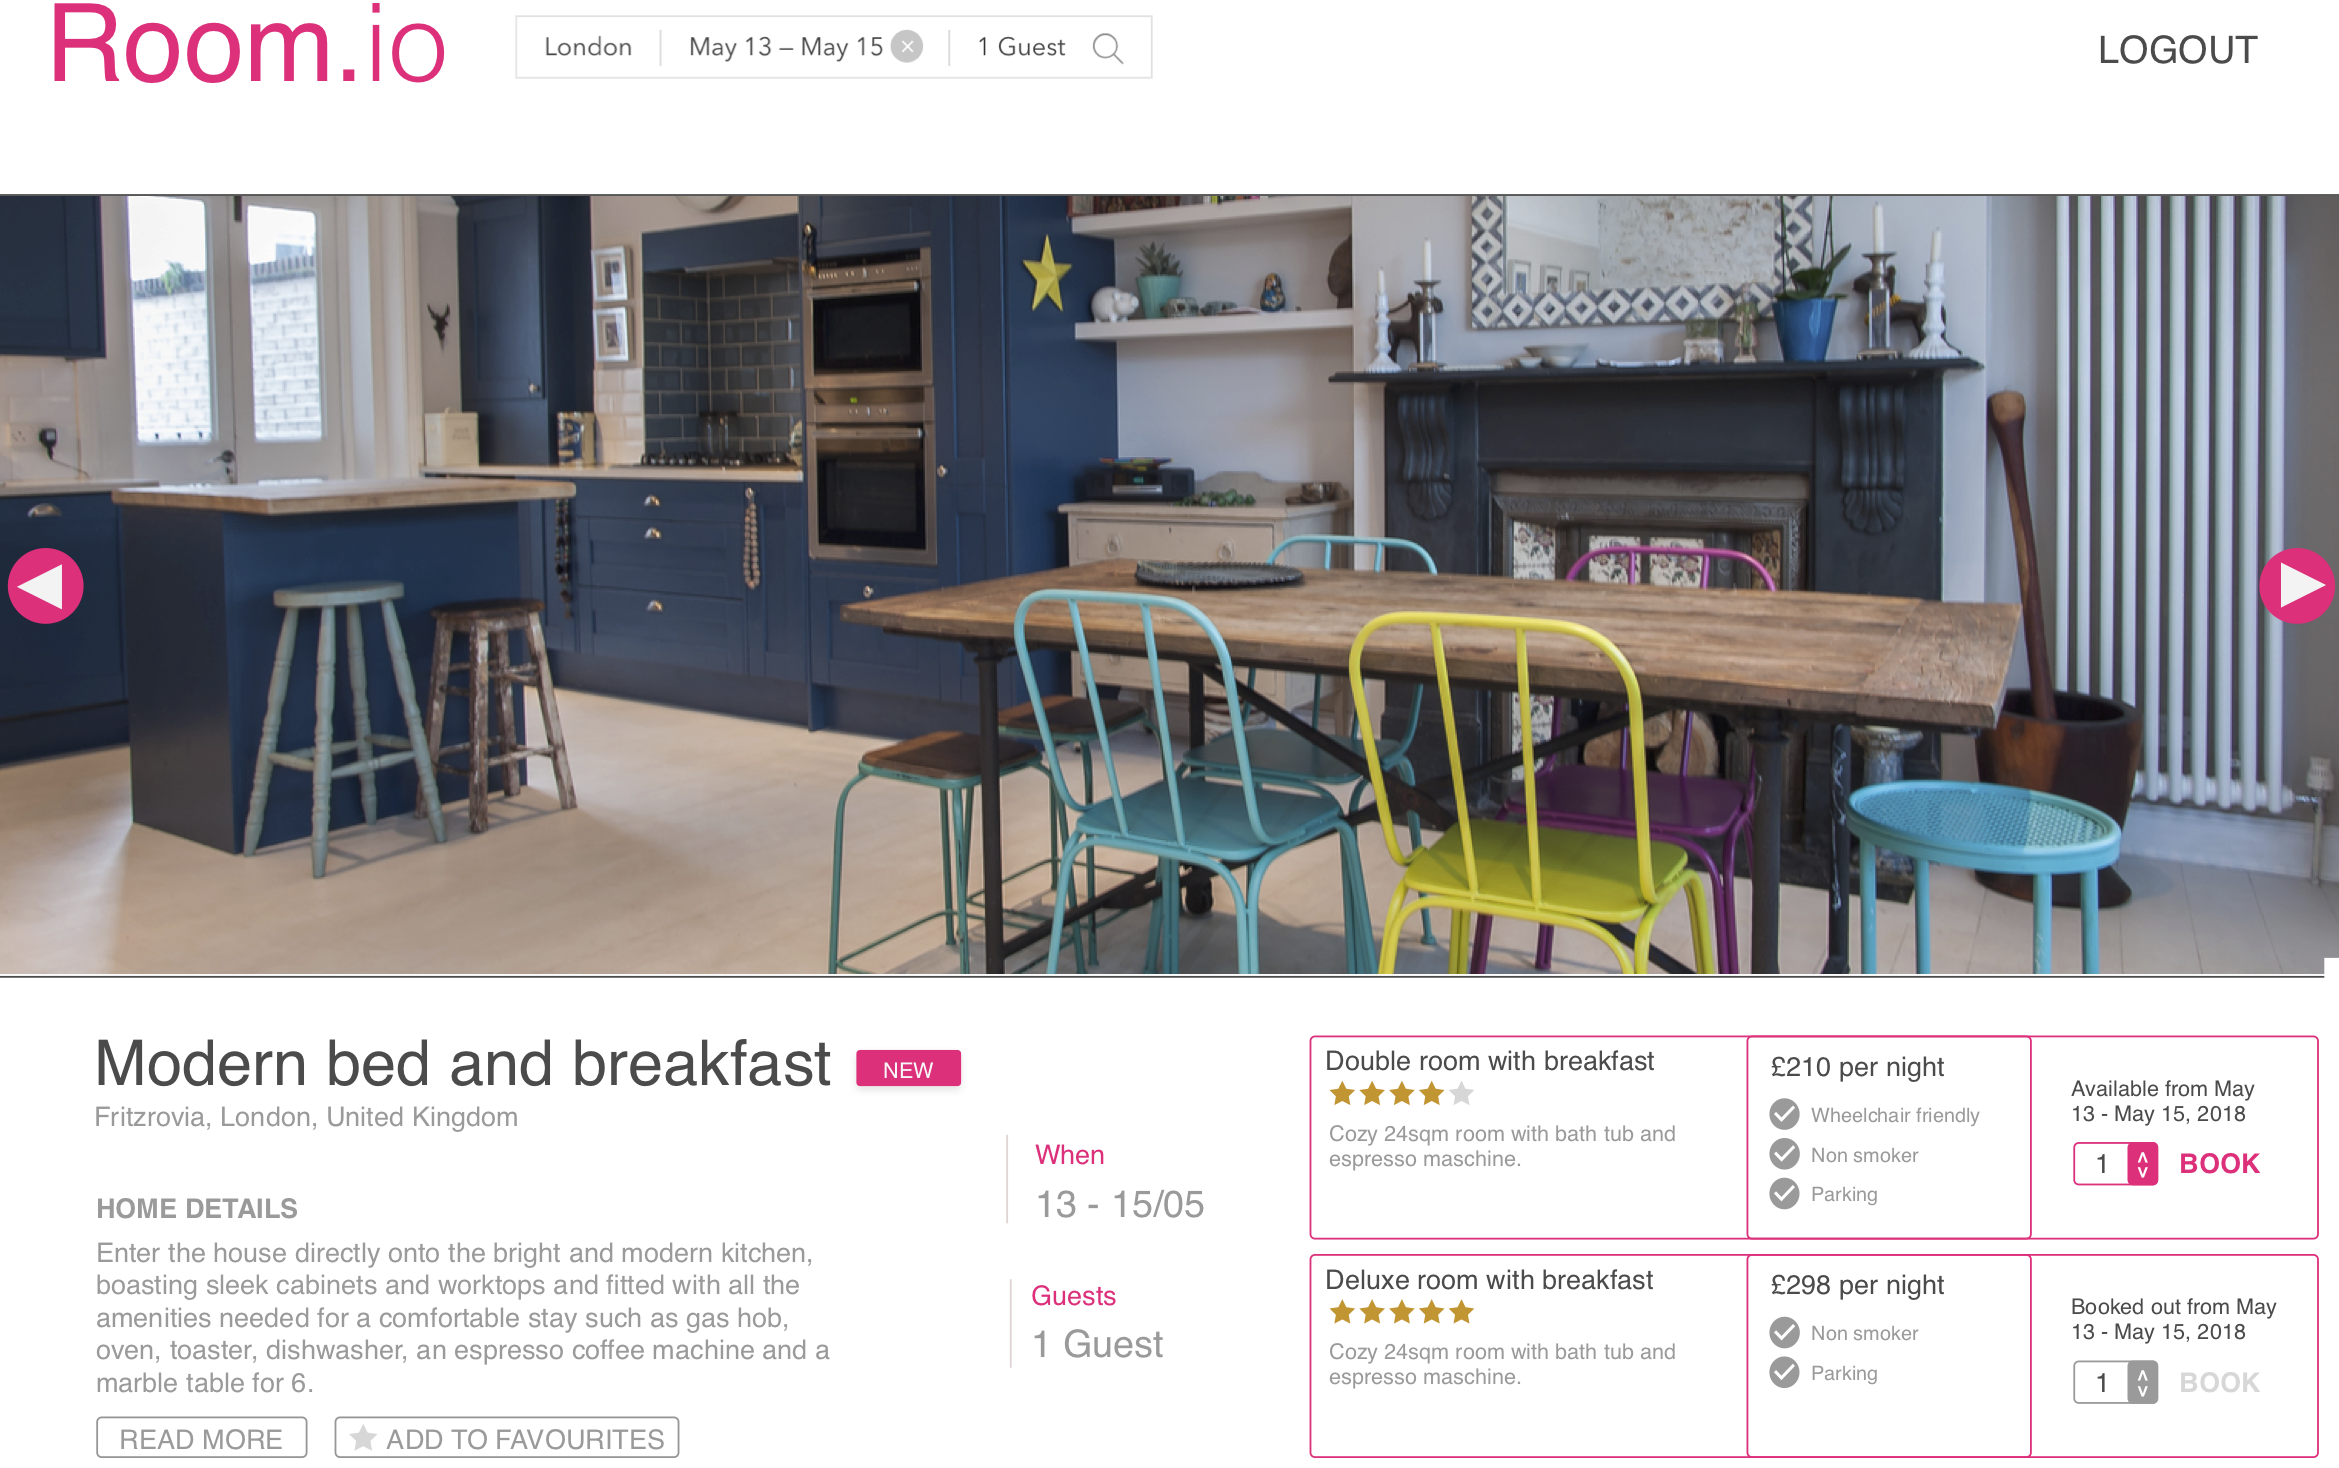
\includegraphics[width=17cm]{img/mockups/guest_detailedproperty.png}
  \caption{Detailed property view}
  \label{Property_List_View}
\end{figure}

\begin{figure}[H]
  \centering
  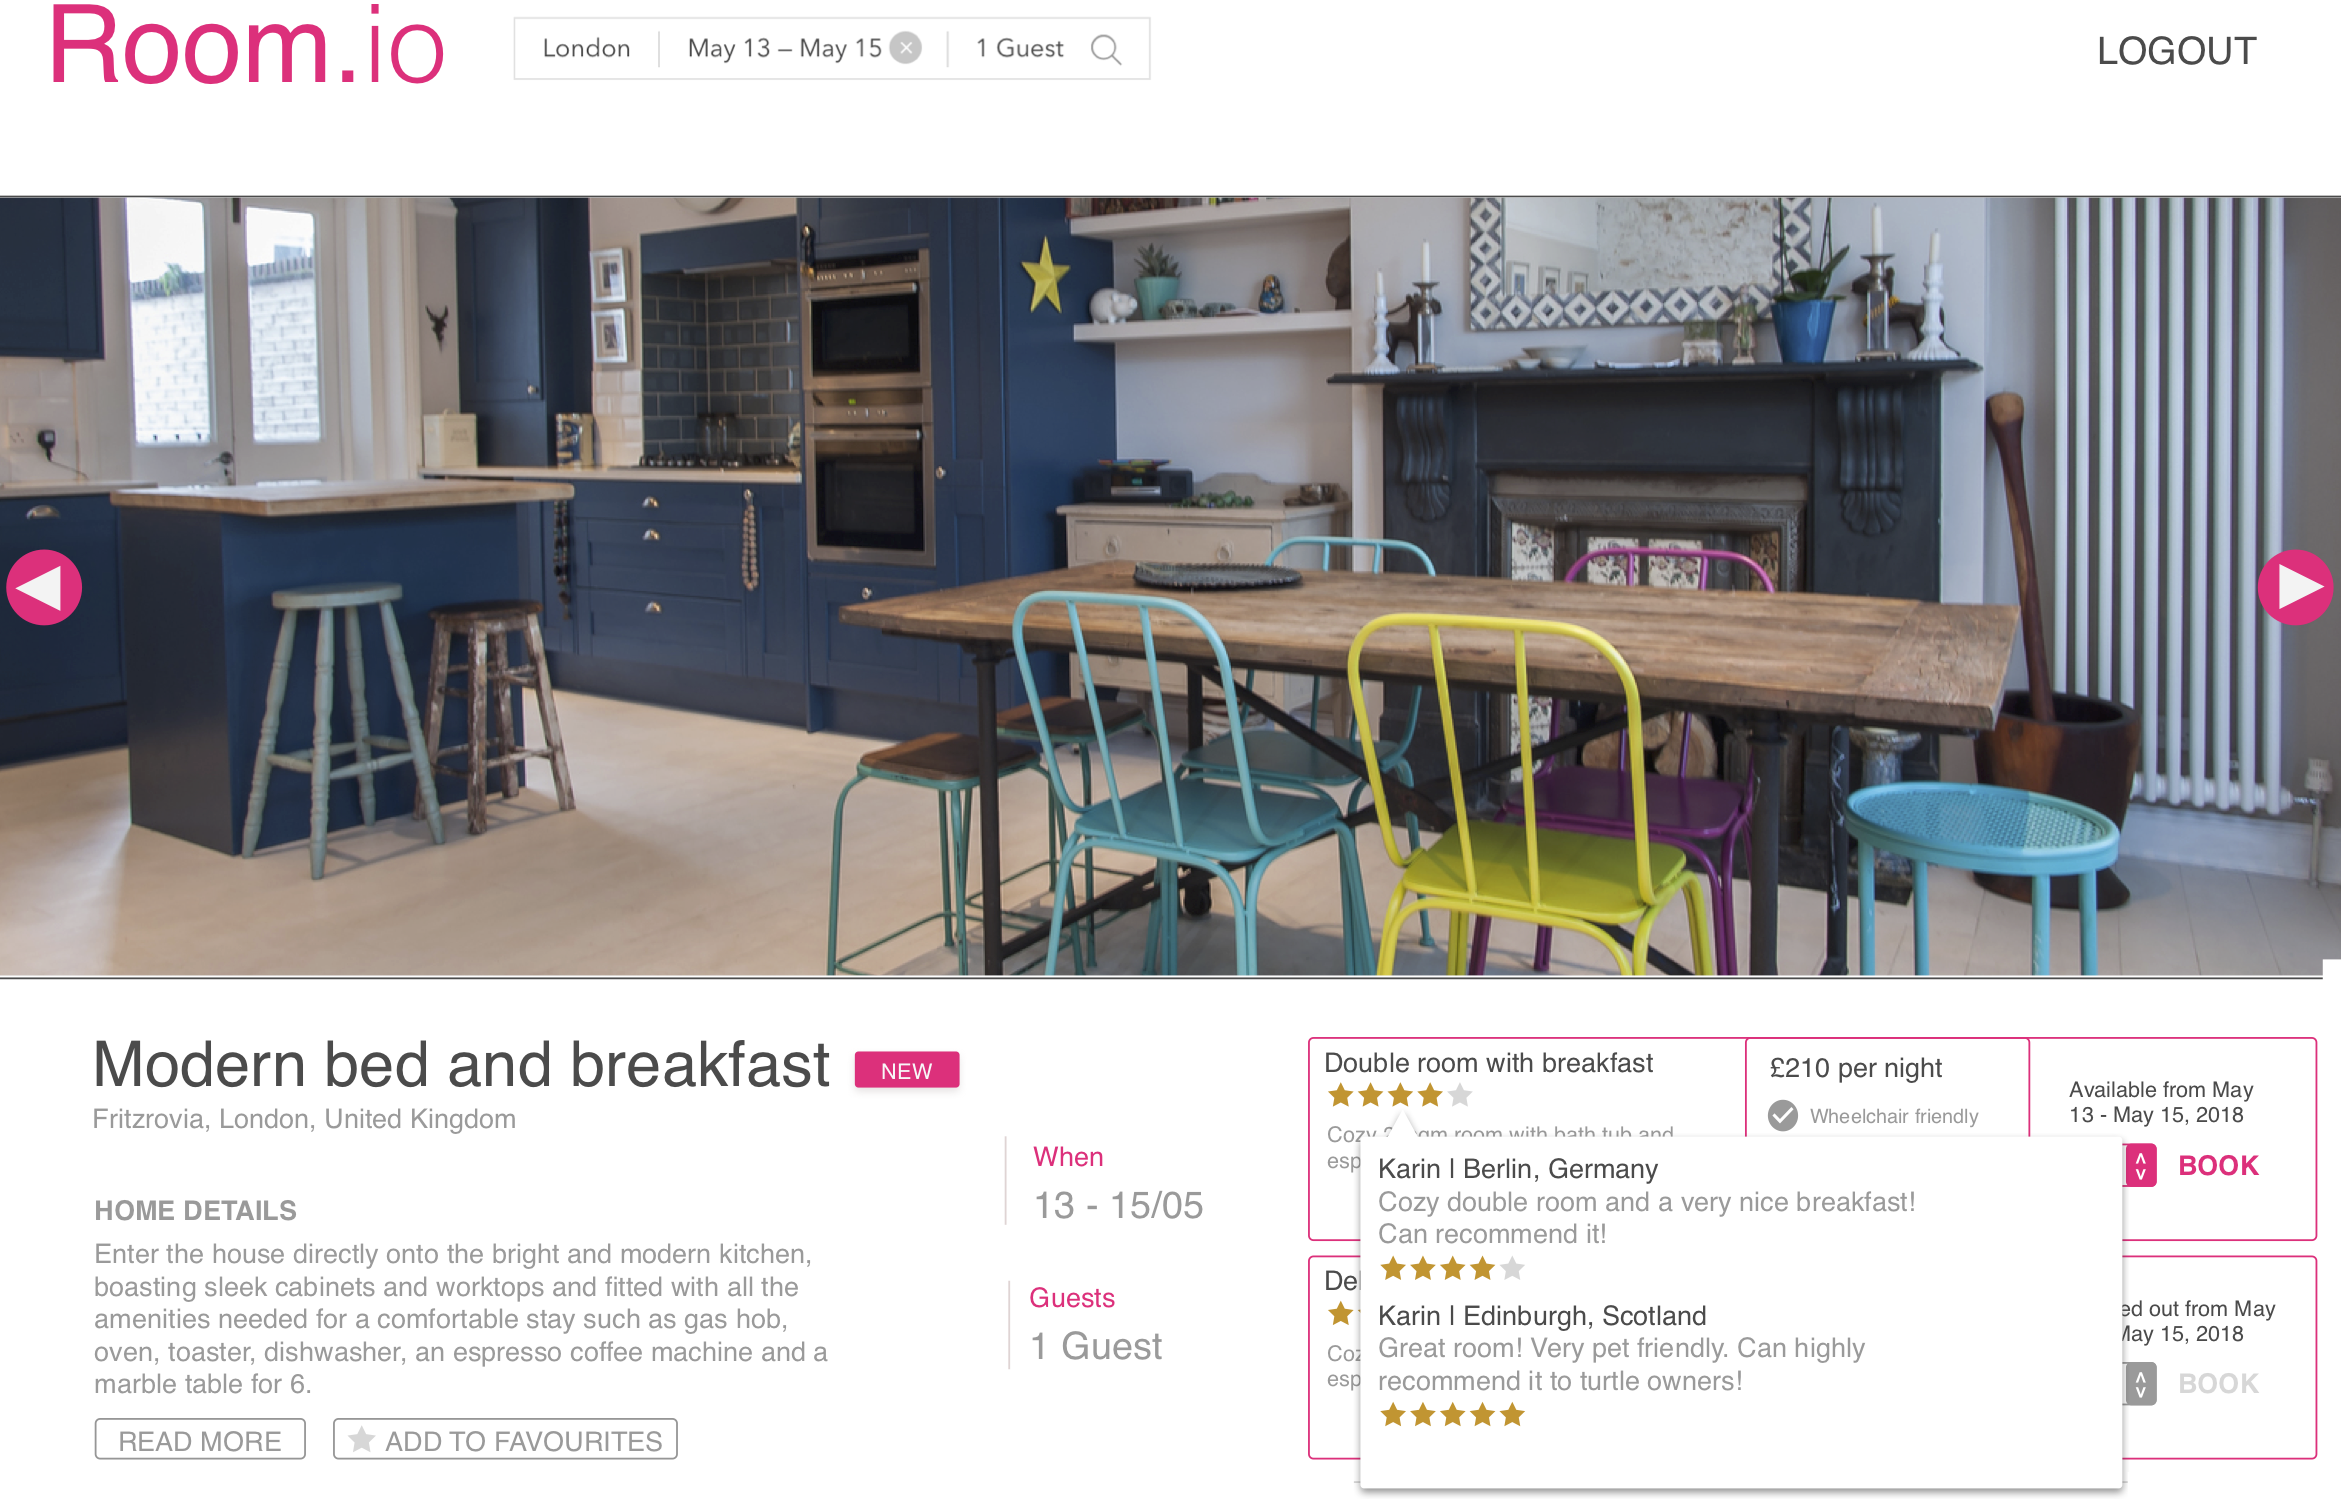
\includegraphics[width=17cm]{img/mockups/guest_detailedpropertyratings.png}
  \caption{Detailed property rating view}
  \label{Detailed_Property_Rating_View}
\end{figure}

\subsection{Favourites}
On the "favourites" list the Guest is able to save properties. By clicking on one of these properties, they are directed to the detailed property view. In this view, the Guest can also delete properties from the list by clicking on the "Remove from Favourites" button above each property excerpt.

\begin{figure}[H]
  \centering
  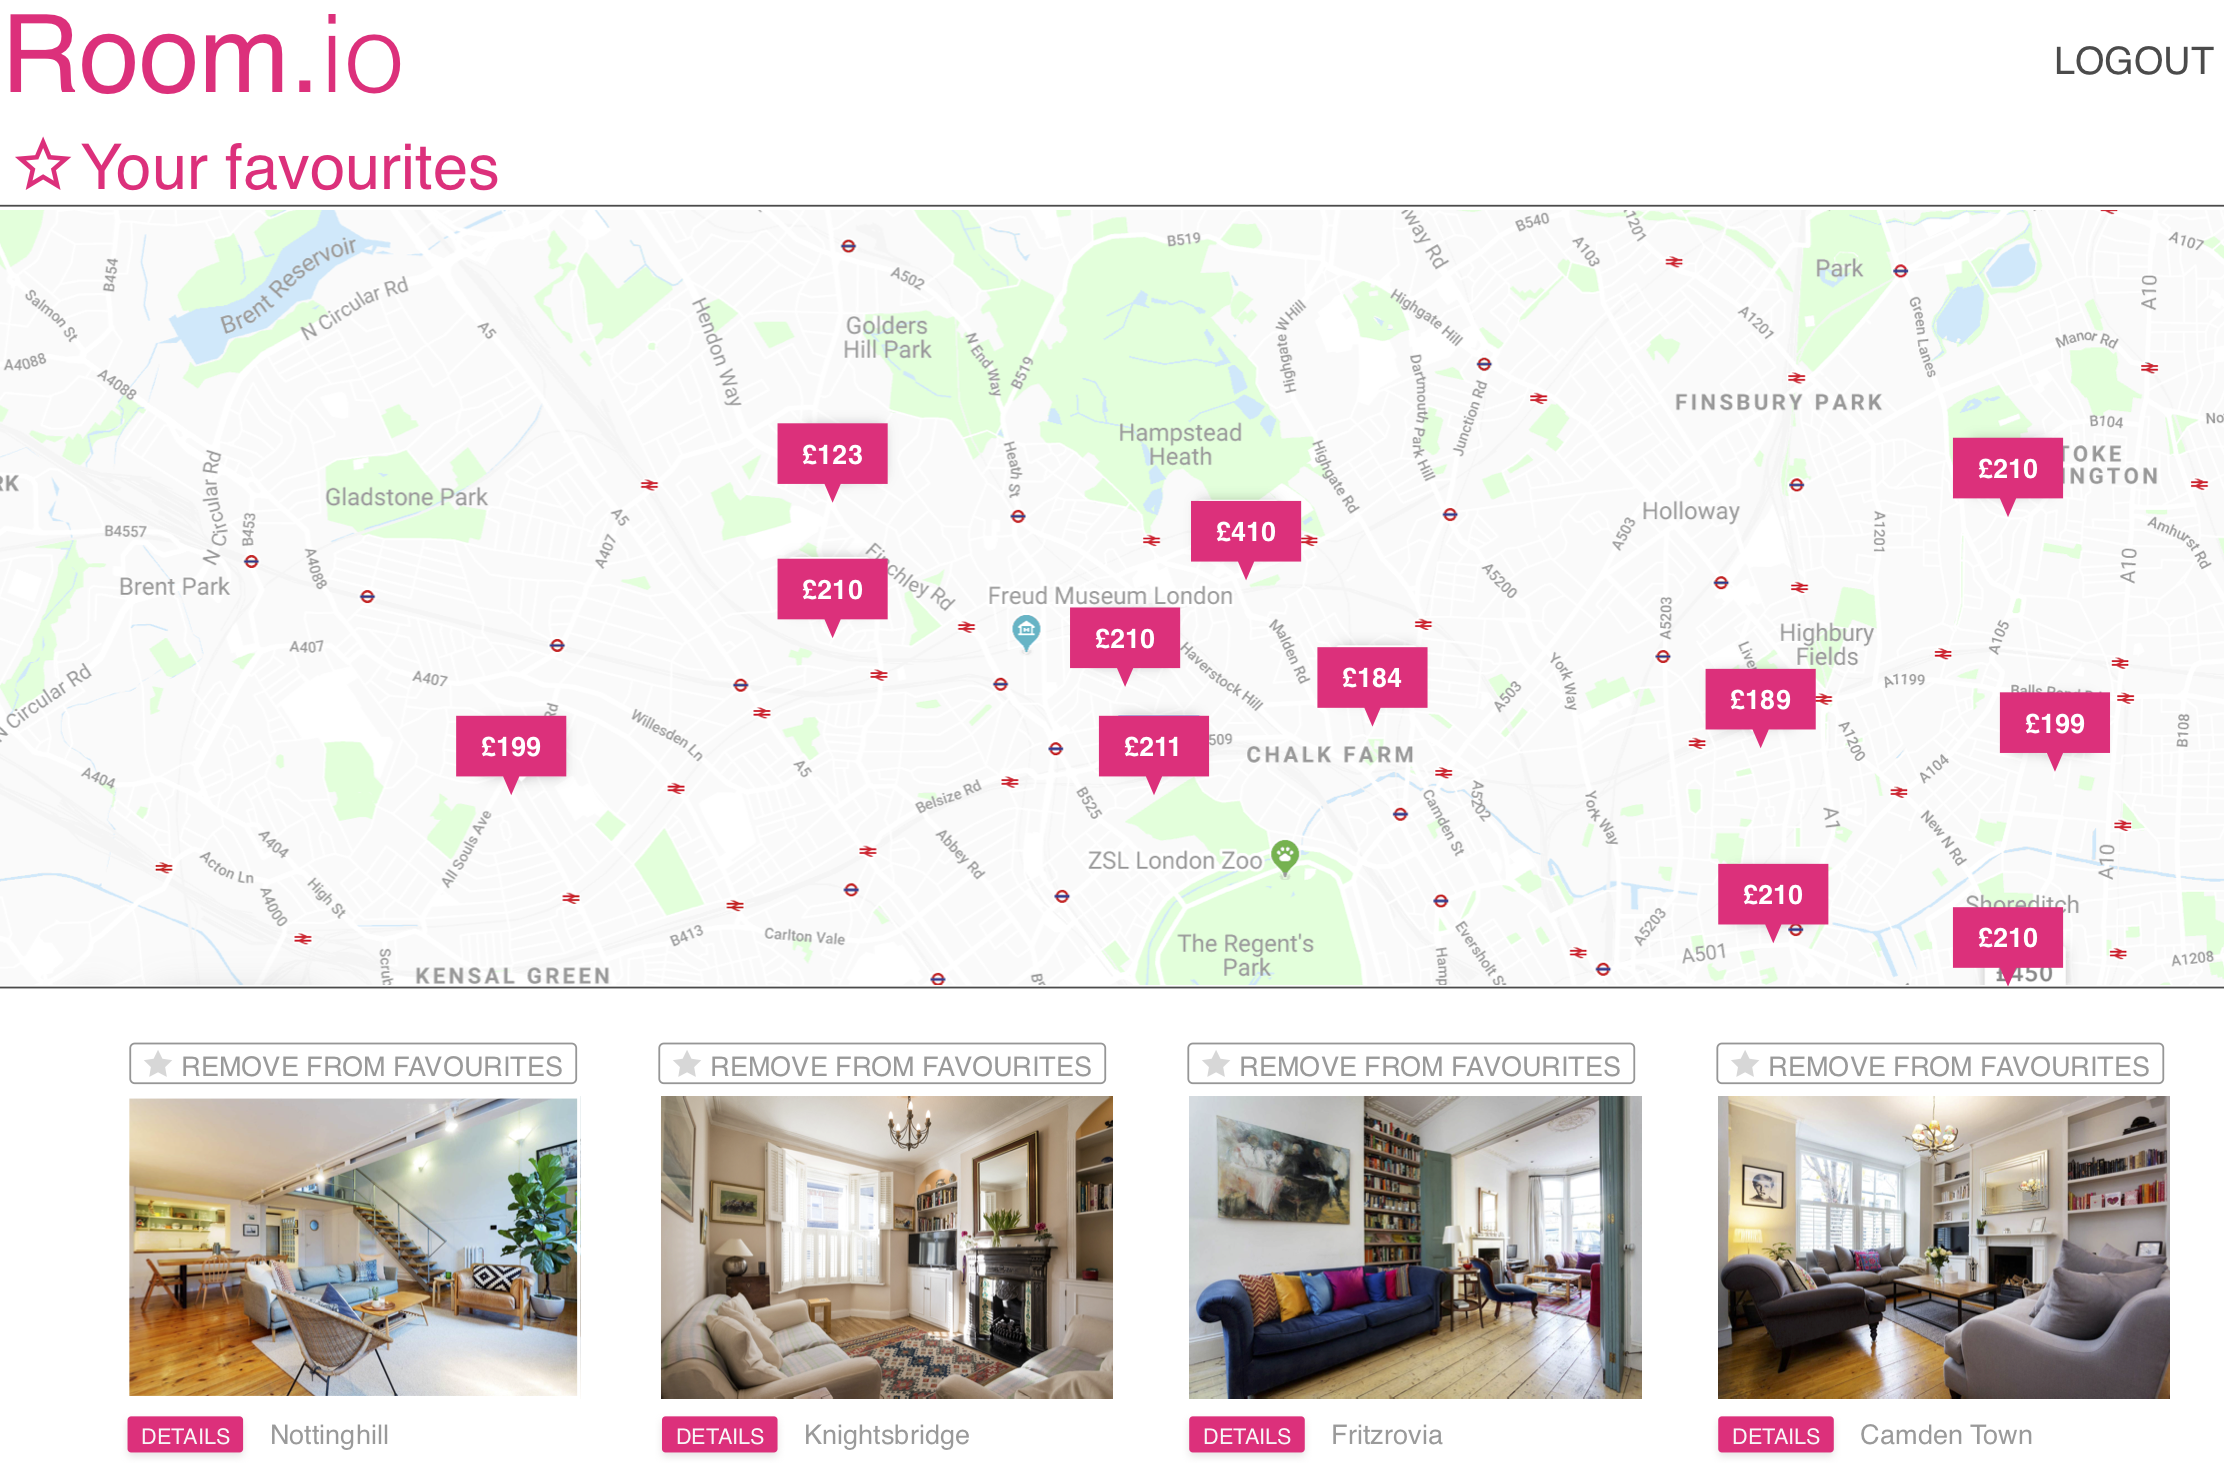
\includegraphics[width=17cm]{img/mockups/guest_favorites.png}
  \caption{Favourites view}
  \label{Favorites_View}
\end{figure}

\subsection{Make a Booking}
After confirming the availability for a chosen room on the detailed property view, the Guest can make a booking for it. To do so, they simply need to indicate their personal details and in a second step fill in their credit card details. If their details are correct, they receive a booking confirmation. If they are not valid, a popup informs them about the incorrect details.

\begin{figure}[H]
  \centering
  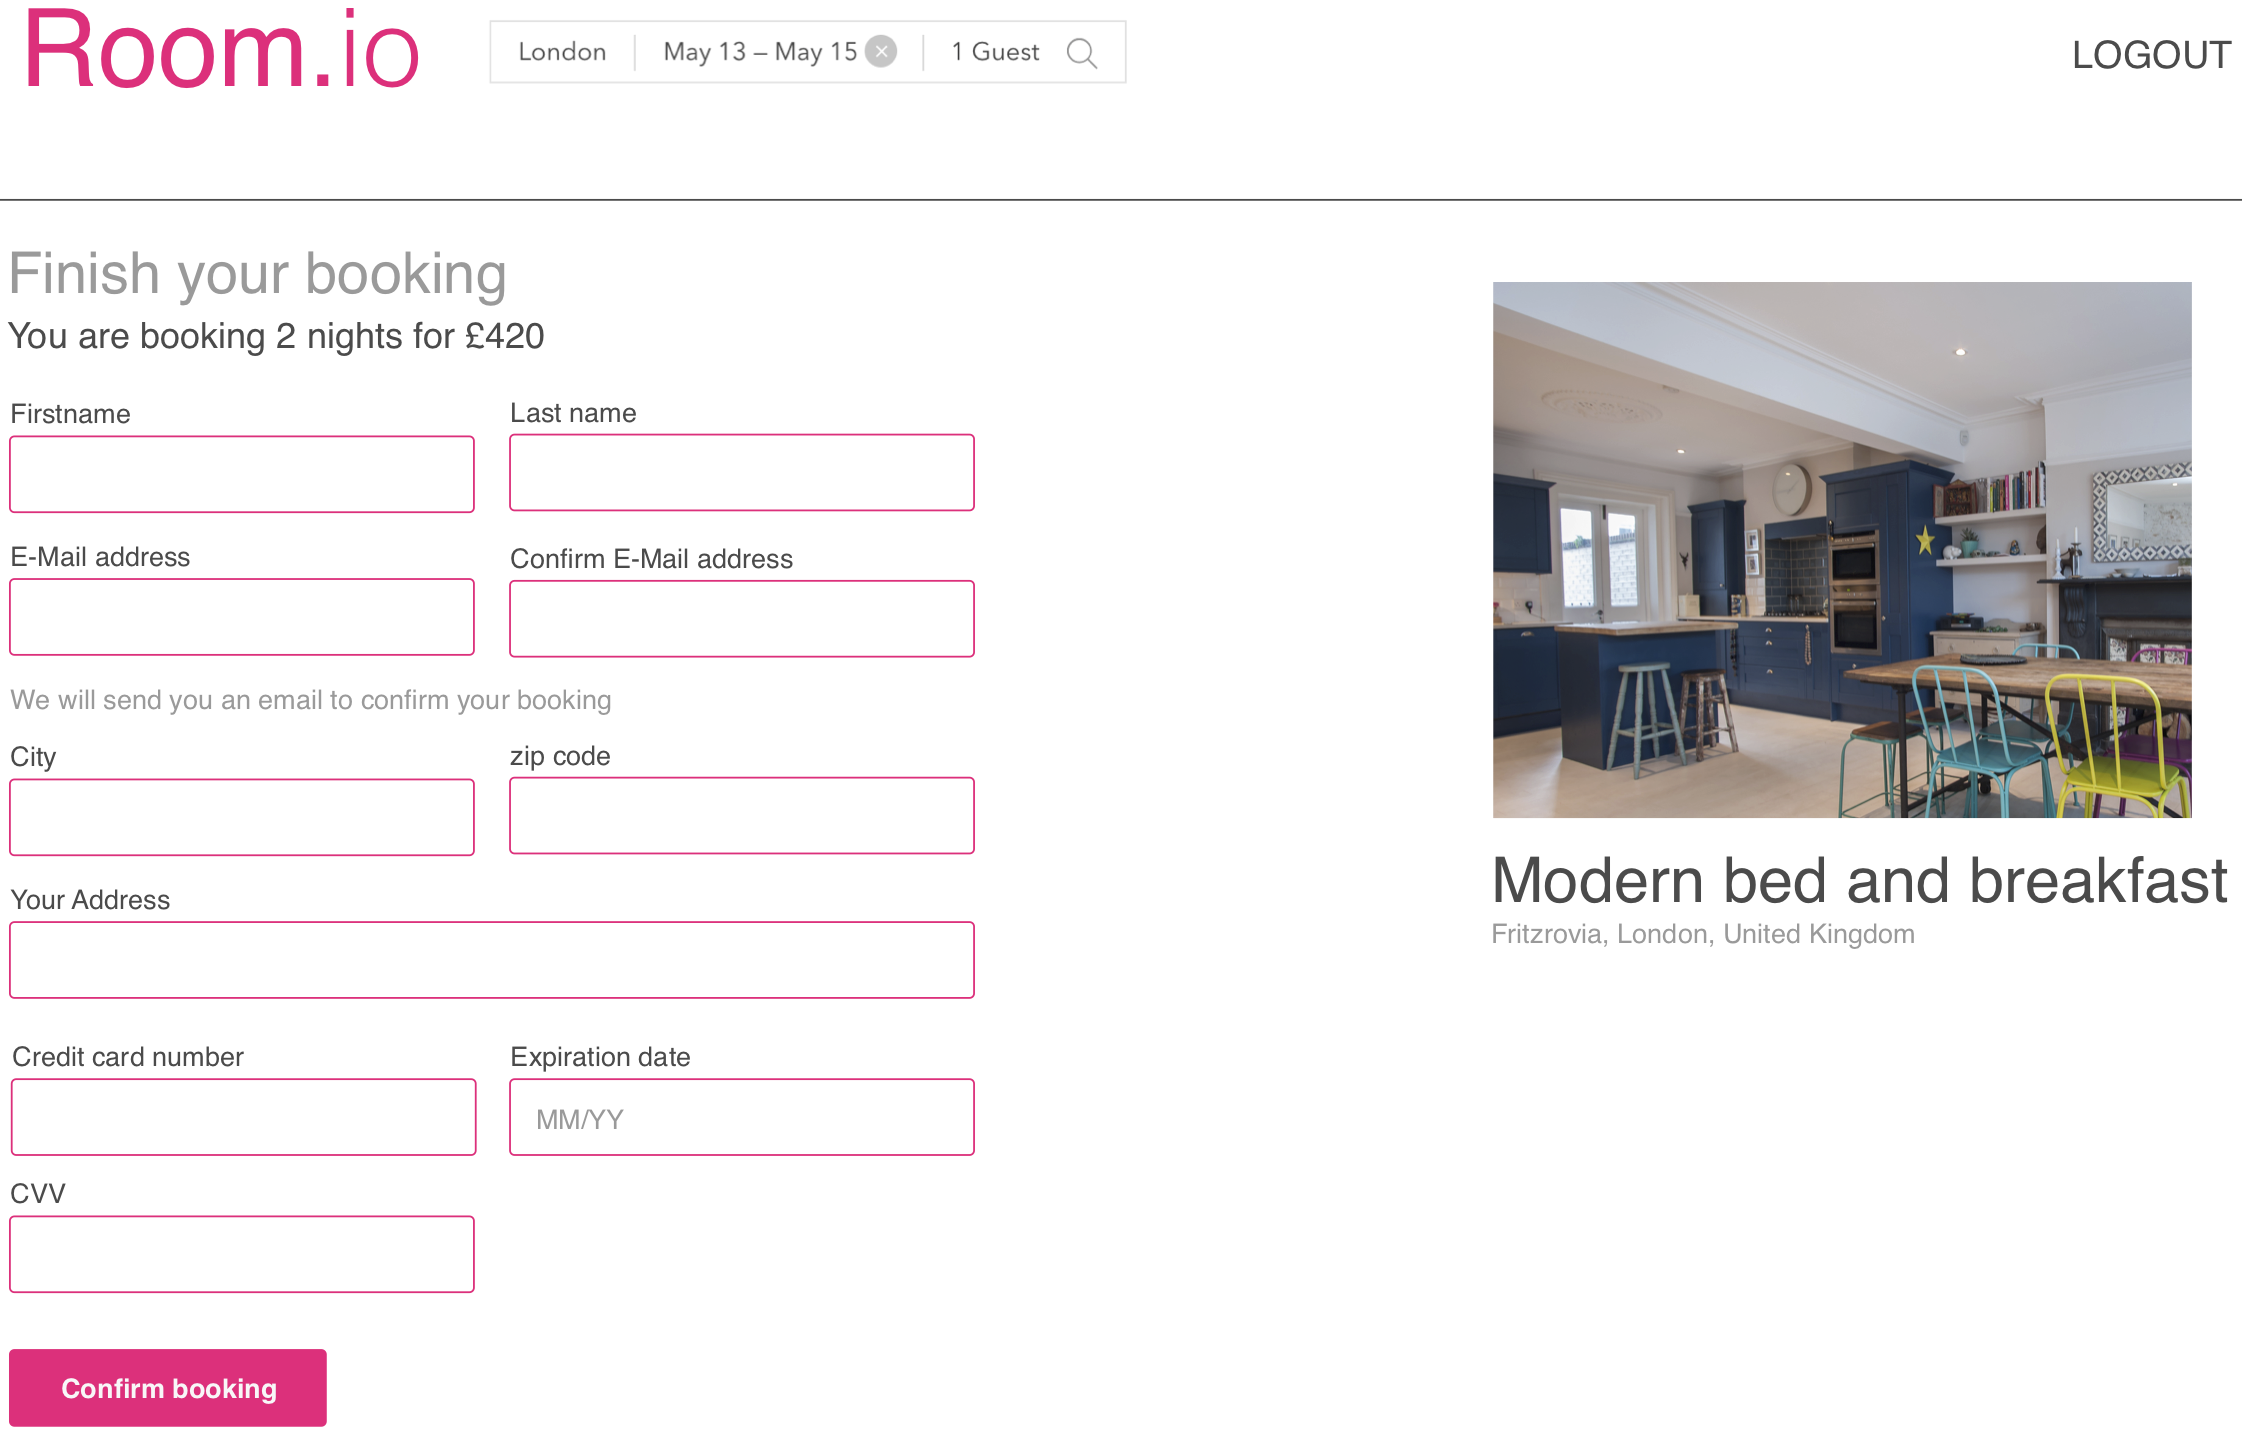
\includegraphics[width=17cm]{img/mockups/guest_booking.png}
  \caption{Booking view}
  \label{Booking_View}
\end{figure}

\subsection{Booking History}
From the search site, the Guest can also access their booking history. Here they are able to delete future bookings as well as give a rating for the properties they already visited.

\begin{figure}[H]
  \centering
  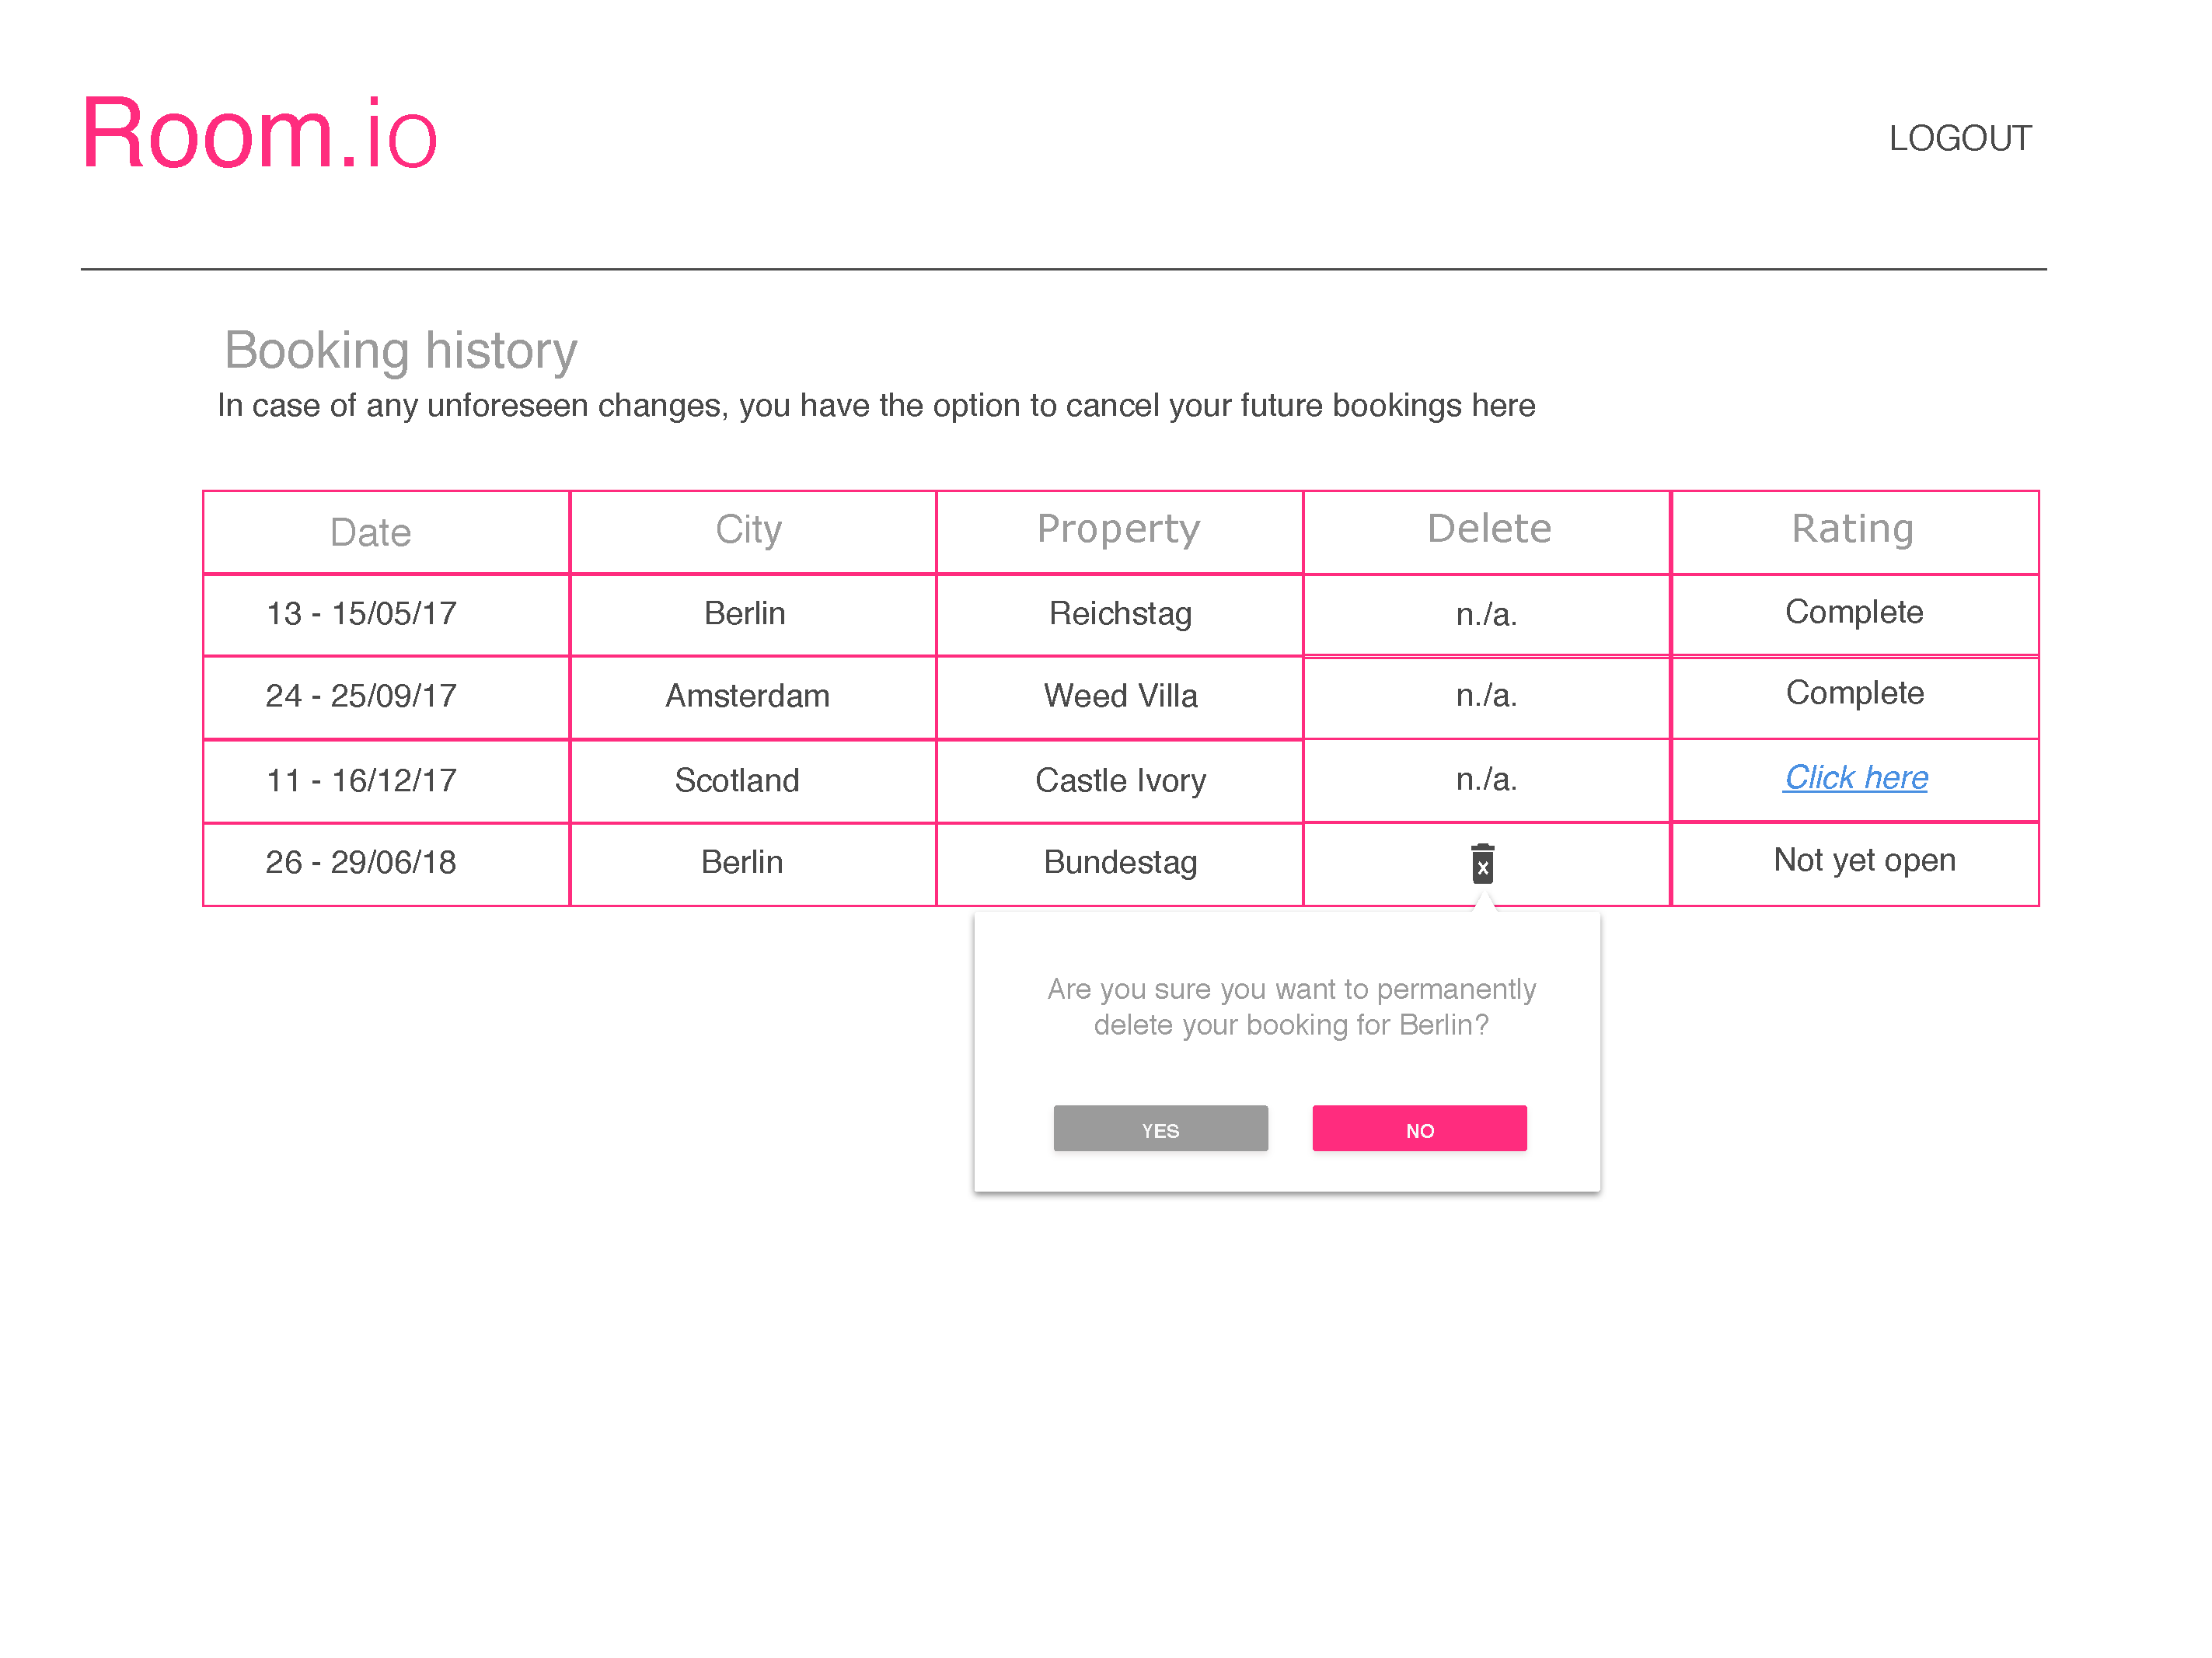
\includegraphics[height=9cm]{img/mockups/guest_bookinghistory.pdf}
  \caption{Booking history}
  \label{Booking_History_View}
\end{figure}

Additionally, they can view their booking history and are able to delete future bookings from here.

\subsection{Give a Rating}
After visiting a property, the Guest is invited to leave a rating for the room they stayed at. To do so, they need to rank their stay by assigning stars in the range from 1 to 5 with 5 being the best. Optionally, they can also add a comment with a header to their review. They are later able to change this feedback by reviewing the property again. 

\begin{figure}[H]
  \centering
  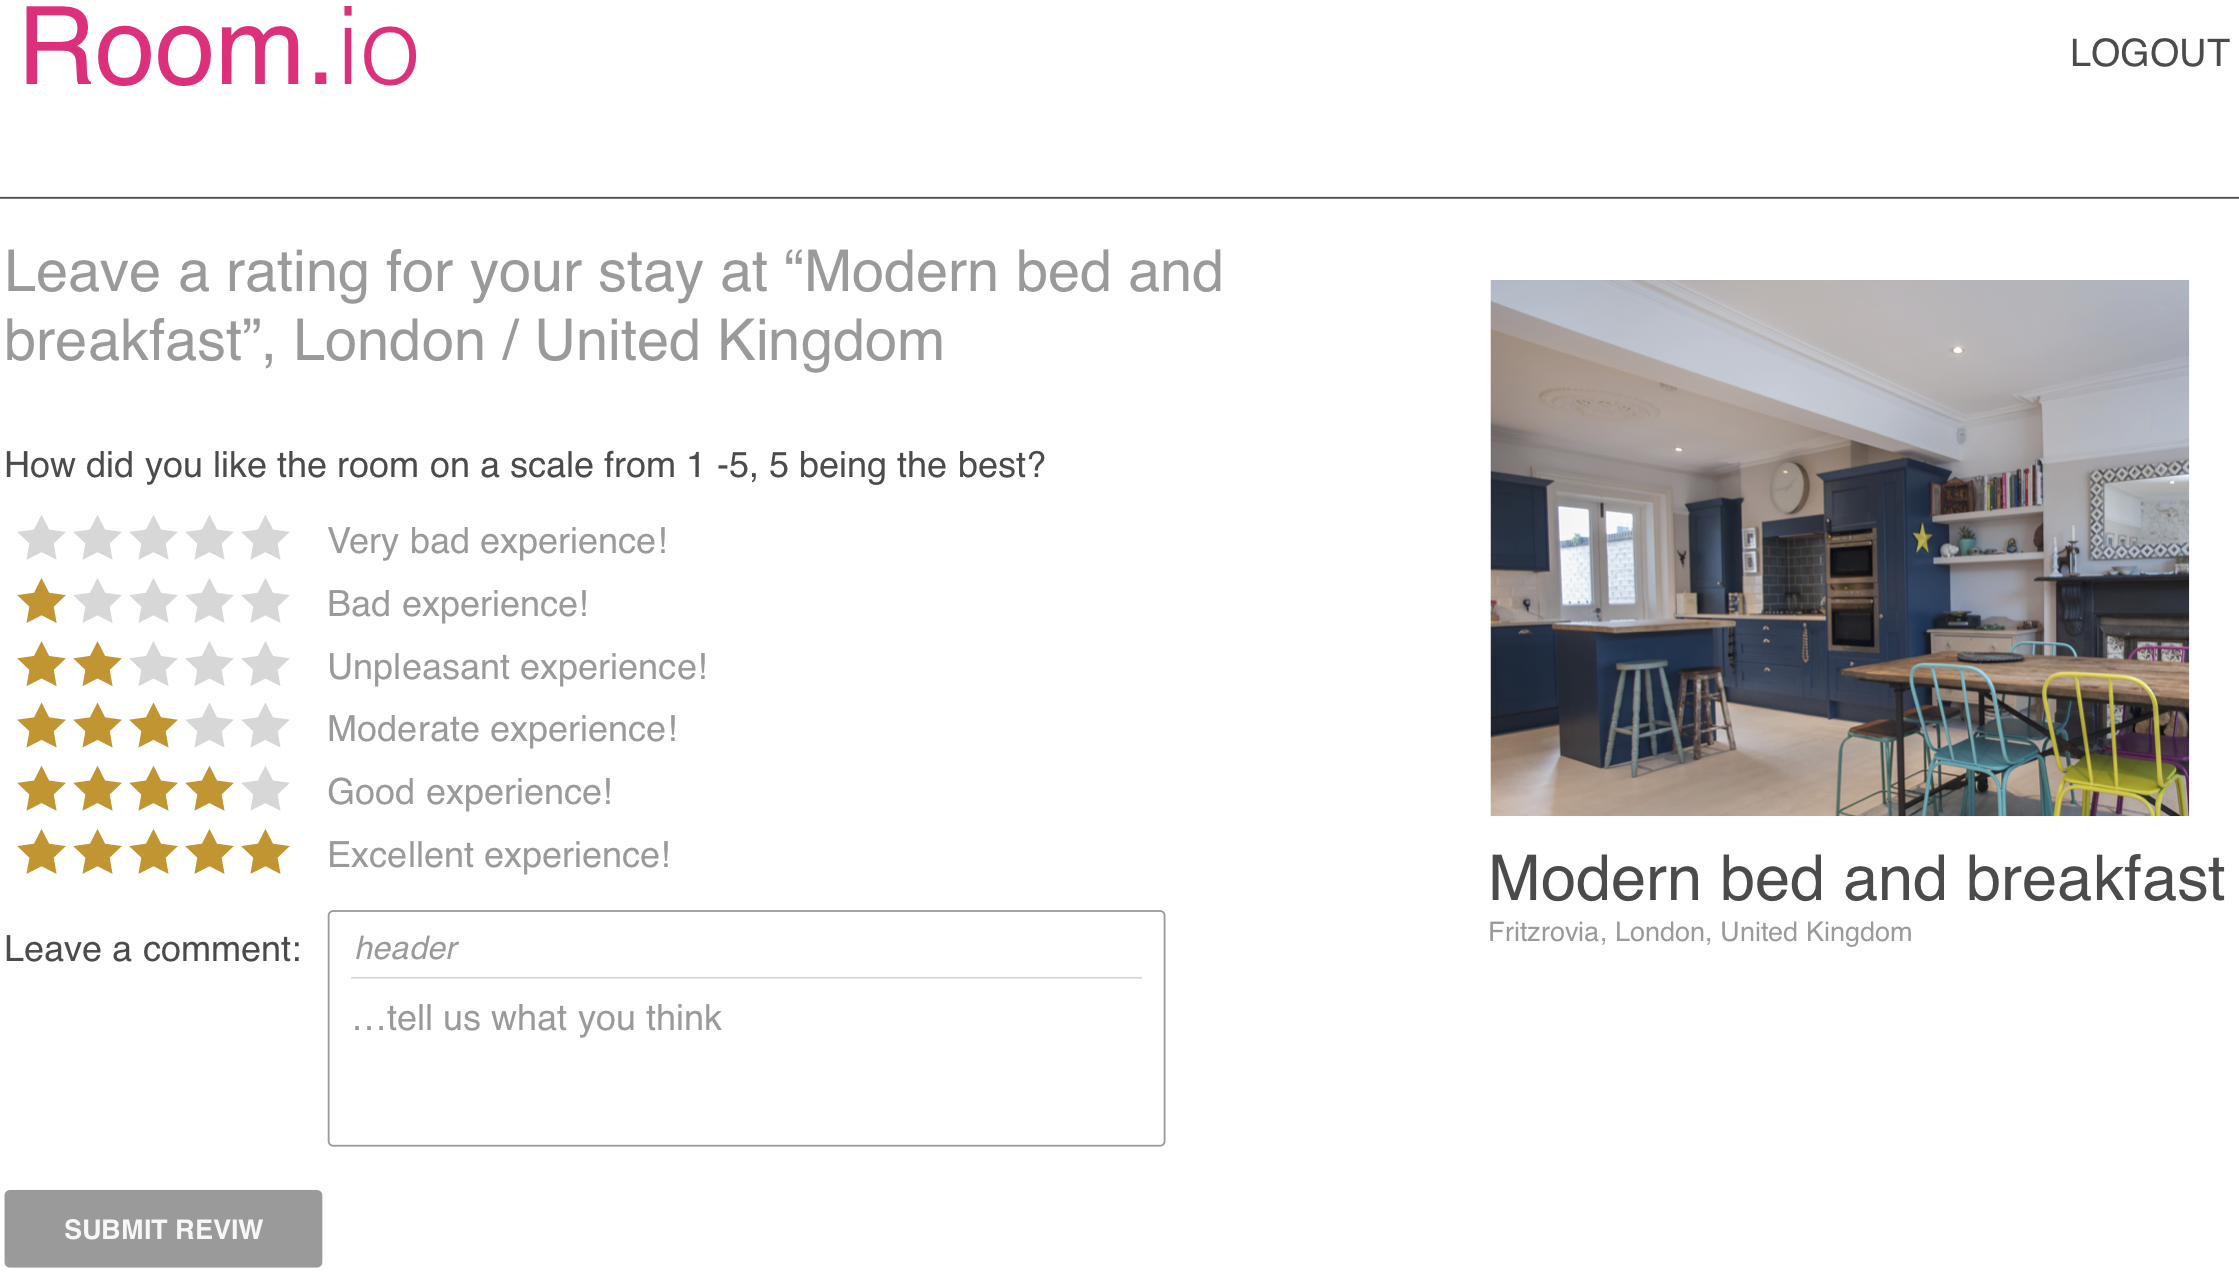
\includegraphics[width=17cm]{img/mockups/guest_rating.png}
  \caption{Rating view}
  \label{Rating_View}
\end{figure}

% ==============================================================================
%                              HOST VIEWS SECTION 
% ==============================================================================
\section{Host Views}
\subsection{Host Dashboard}
If the Host registered a property already, they see an overview of the rooms they currently host in their property together with the future bookings for these. From here they have the option to delete a room, see a preview or edit a room. If no property is registered so far, the Host has the option to add one.

\begin{figure}[H]
  \centering
  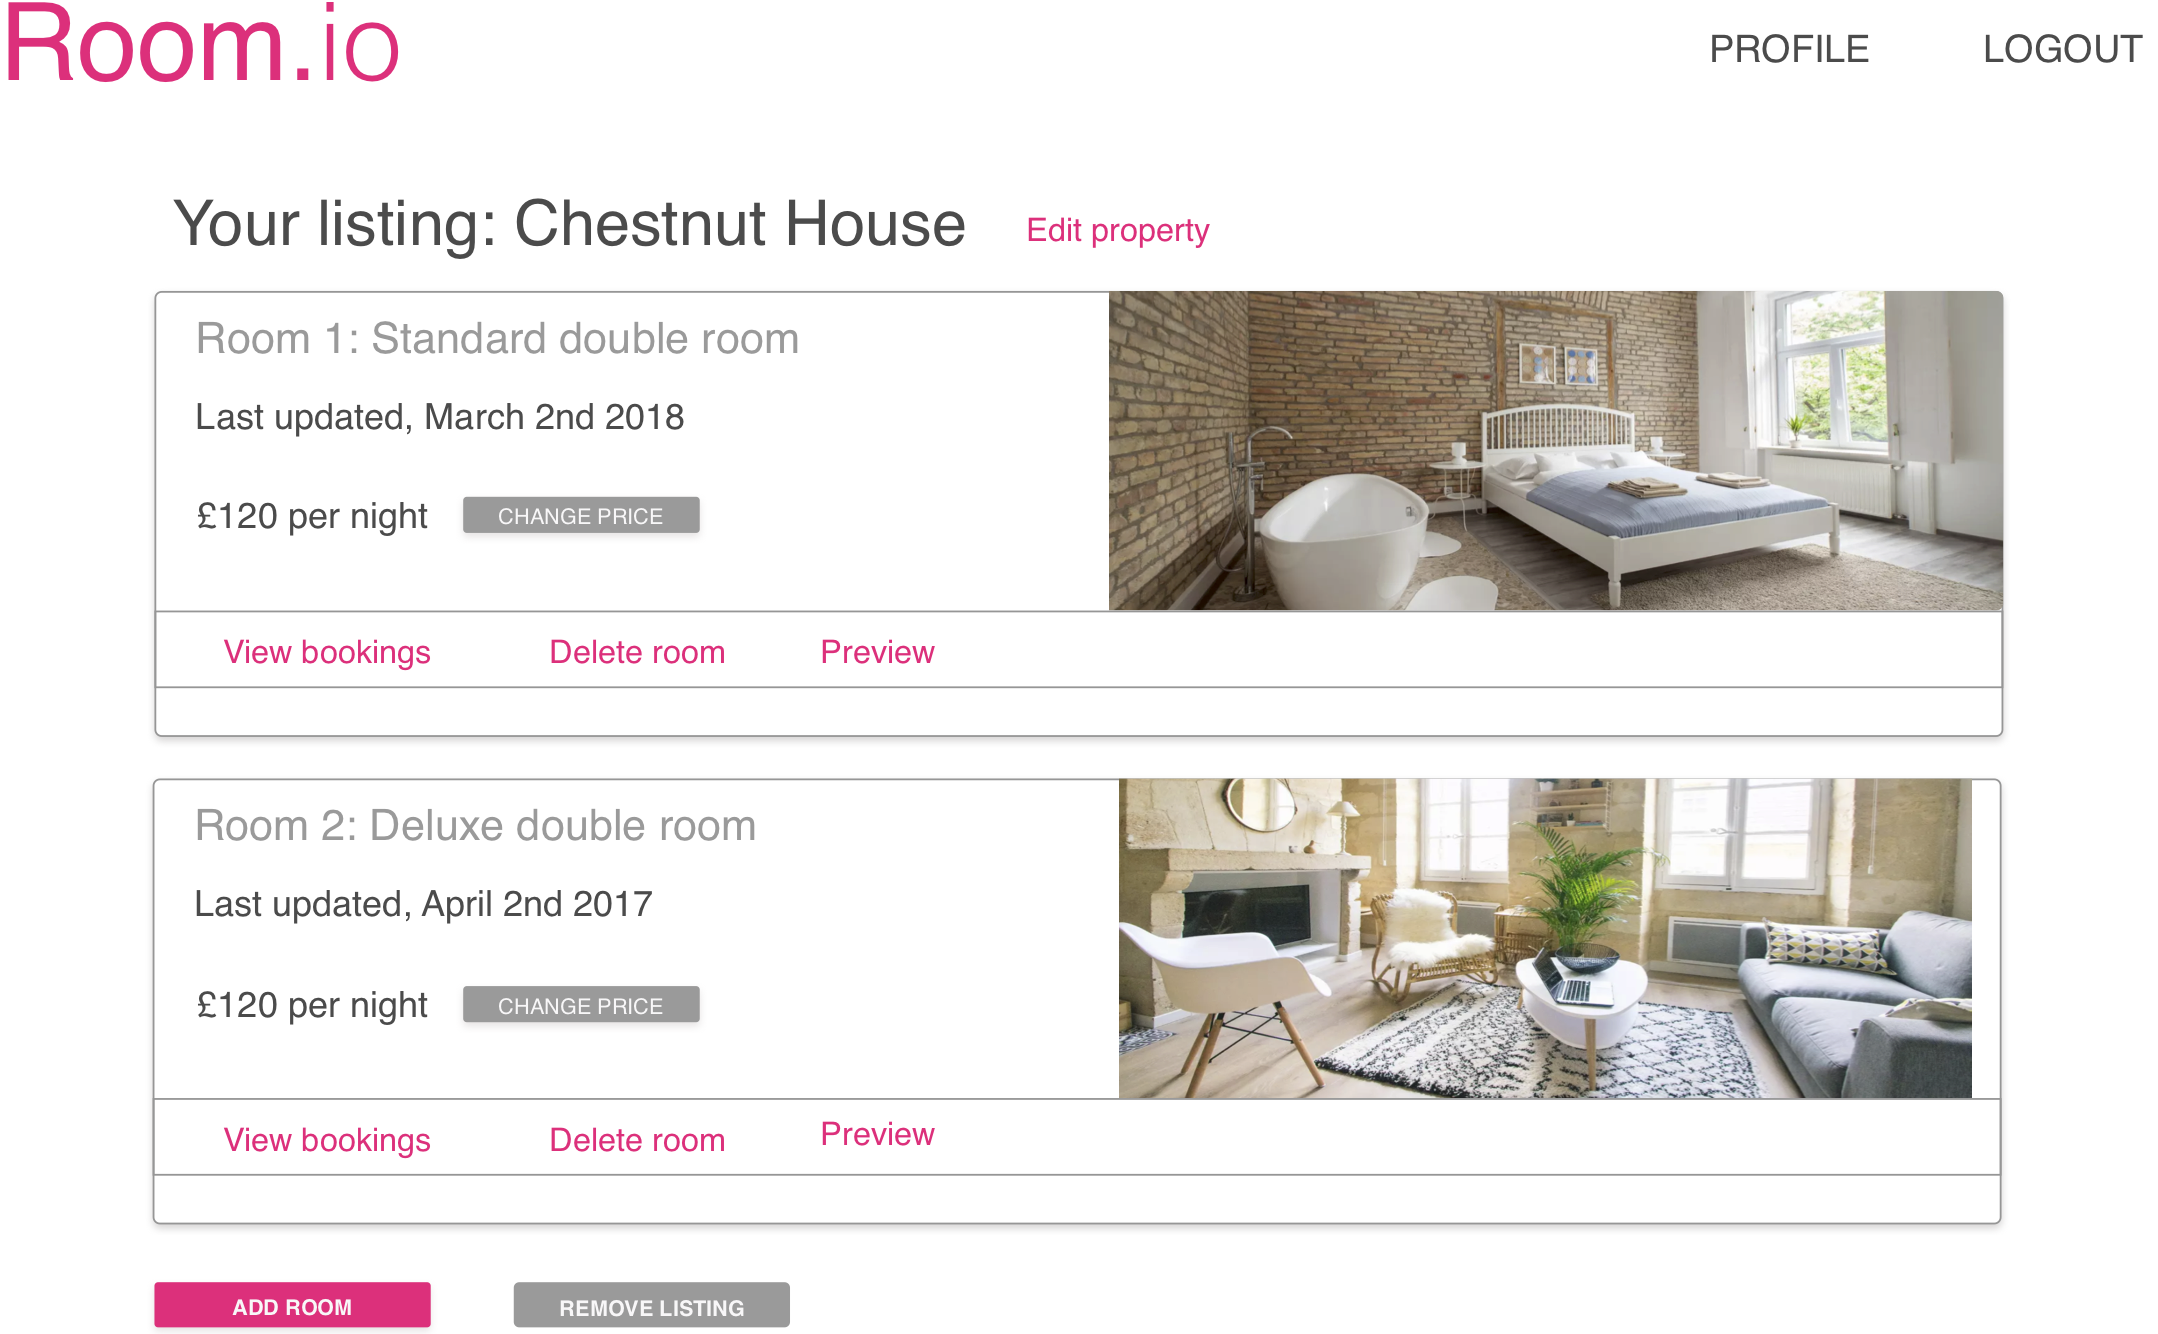
\includegraphics[width=17cm]{img/mockups/host_dashboard.png}
  \caption{Host dashboard}
  \label{Host_Dashboard}
\end{figure}

\subsection{Register a Property}
The Host is only able to register one property. When doing so, they are first asked to provide a property description, an address, earliest check-in, latest check-out, and pictures. Then, they are asked to add a room by inserting a short description, a price for one or two guests, the number of beds the room provides and by selecting policy attributes from a list created by the Admin. Thereafter, they have the option to add the next room. Even though the steps are numbered, the User can return to any step by using the menu on the left side and determine the order of filling in their details by themself. The only requirement for submission, in the end, is that the input complies with all validations. 

\subsection{Edit a Property}
When editing a property, the Host has the option to edit the property descriptions and details such as prices, upload new pictures or simply edit an existing room or add a new one.

\begin{figure}[H]
  \begin{tabular}{c}
    \begin{minipage}[b]{0.5\textwidth}
      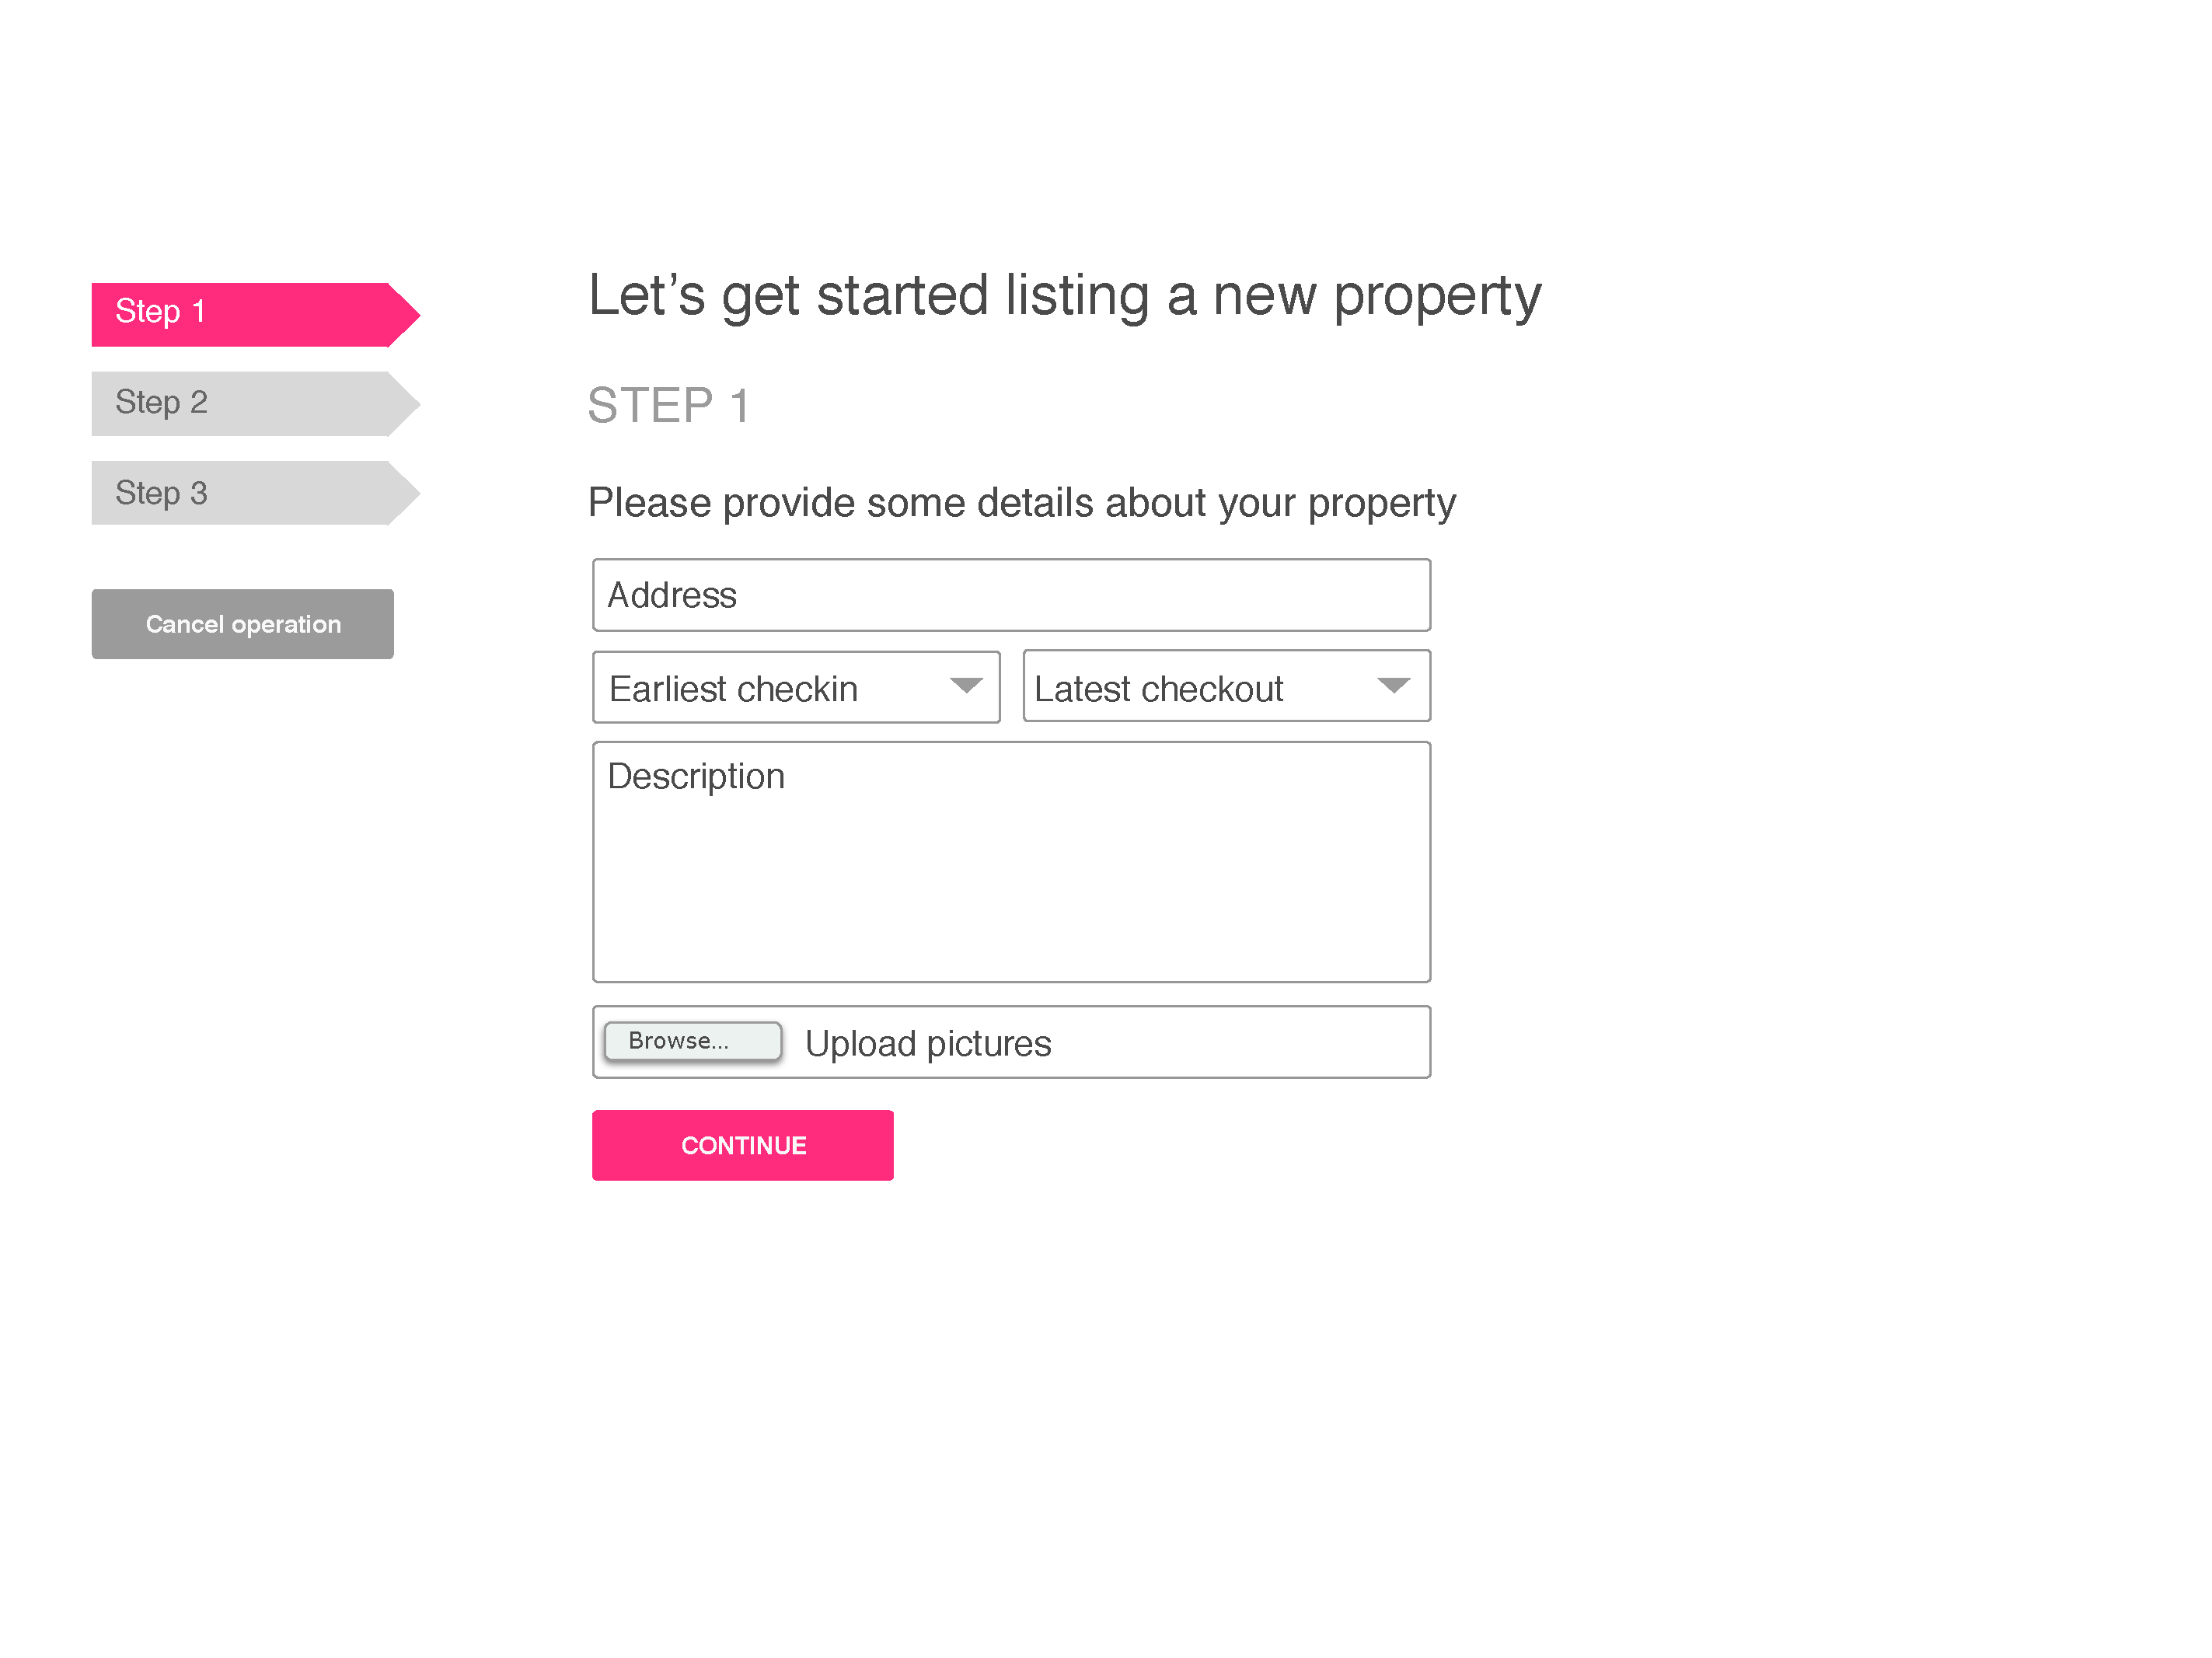
\includegraphics[width=\textwidth]{img/mockups/host_registerproperty1.pdf}
      \caption{Register a property (1/3)}
      \label{register_a_property1}
    \end{minipage}
    \begin{minipage}[b]{0.5\textwidth}
      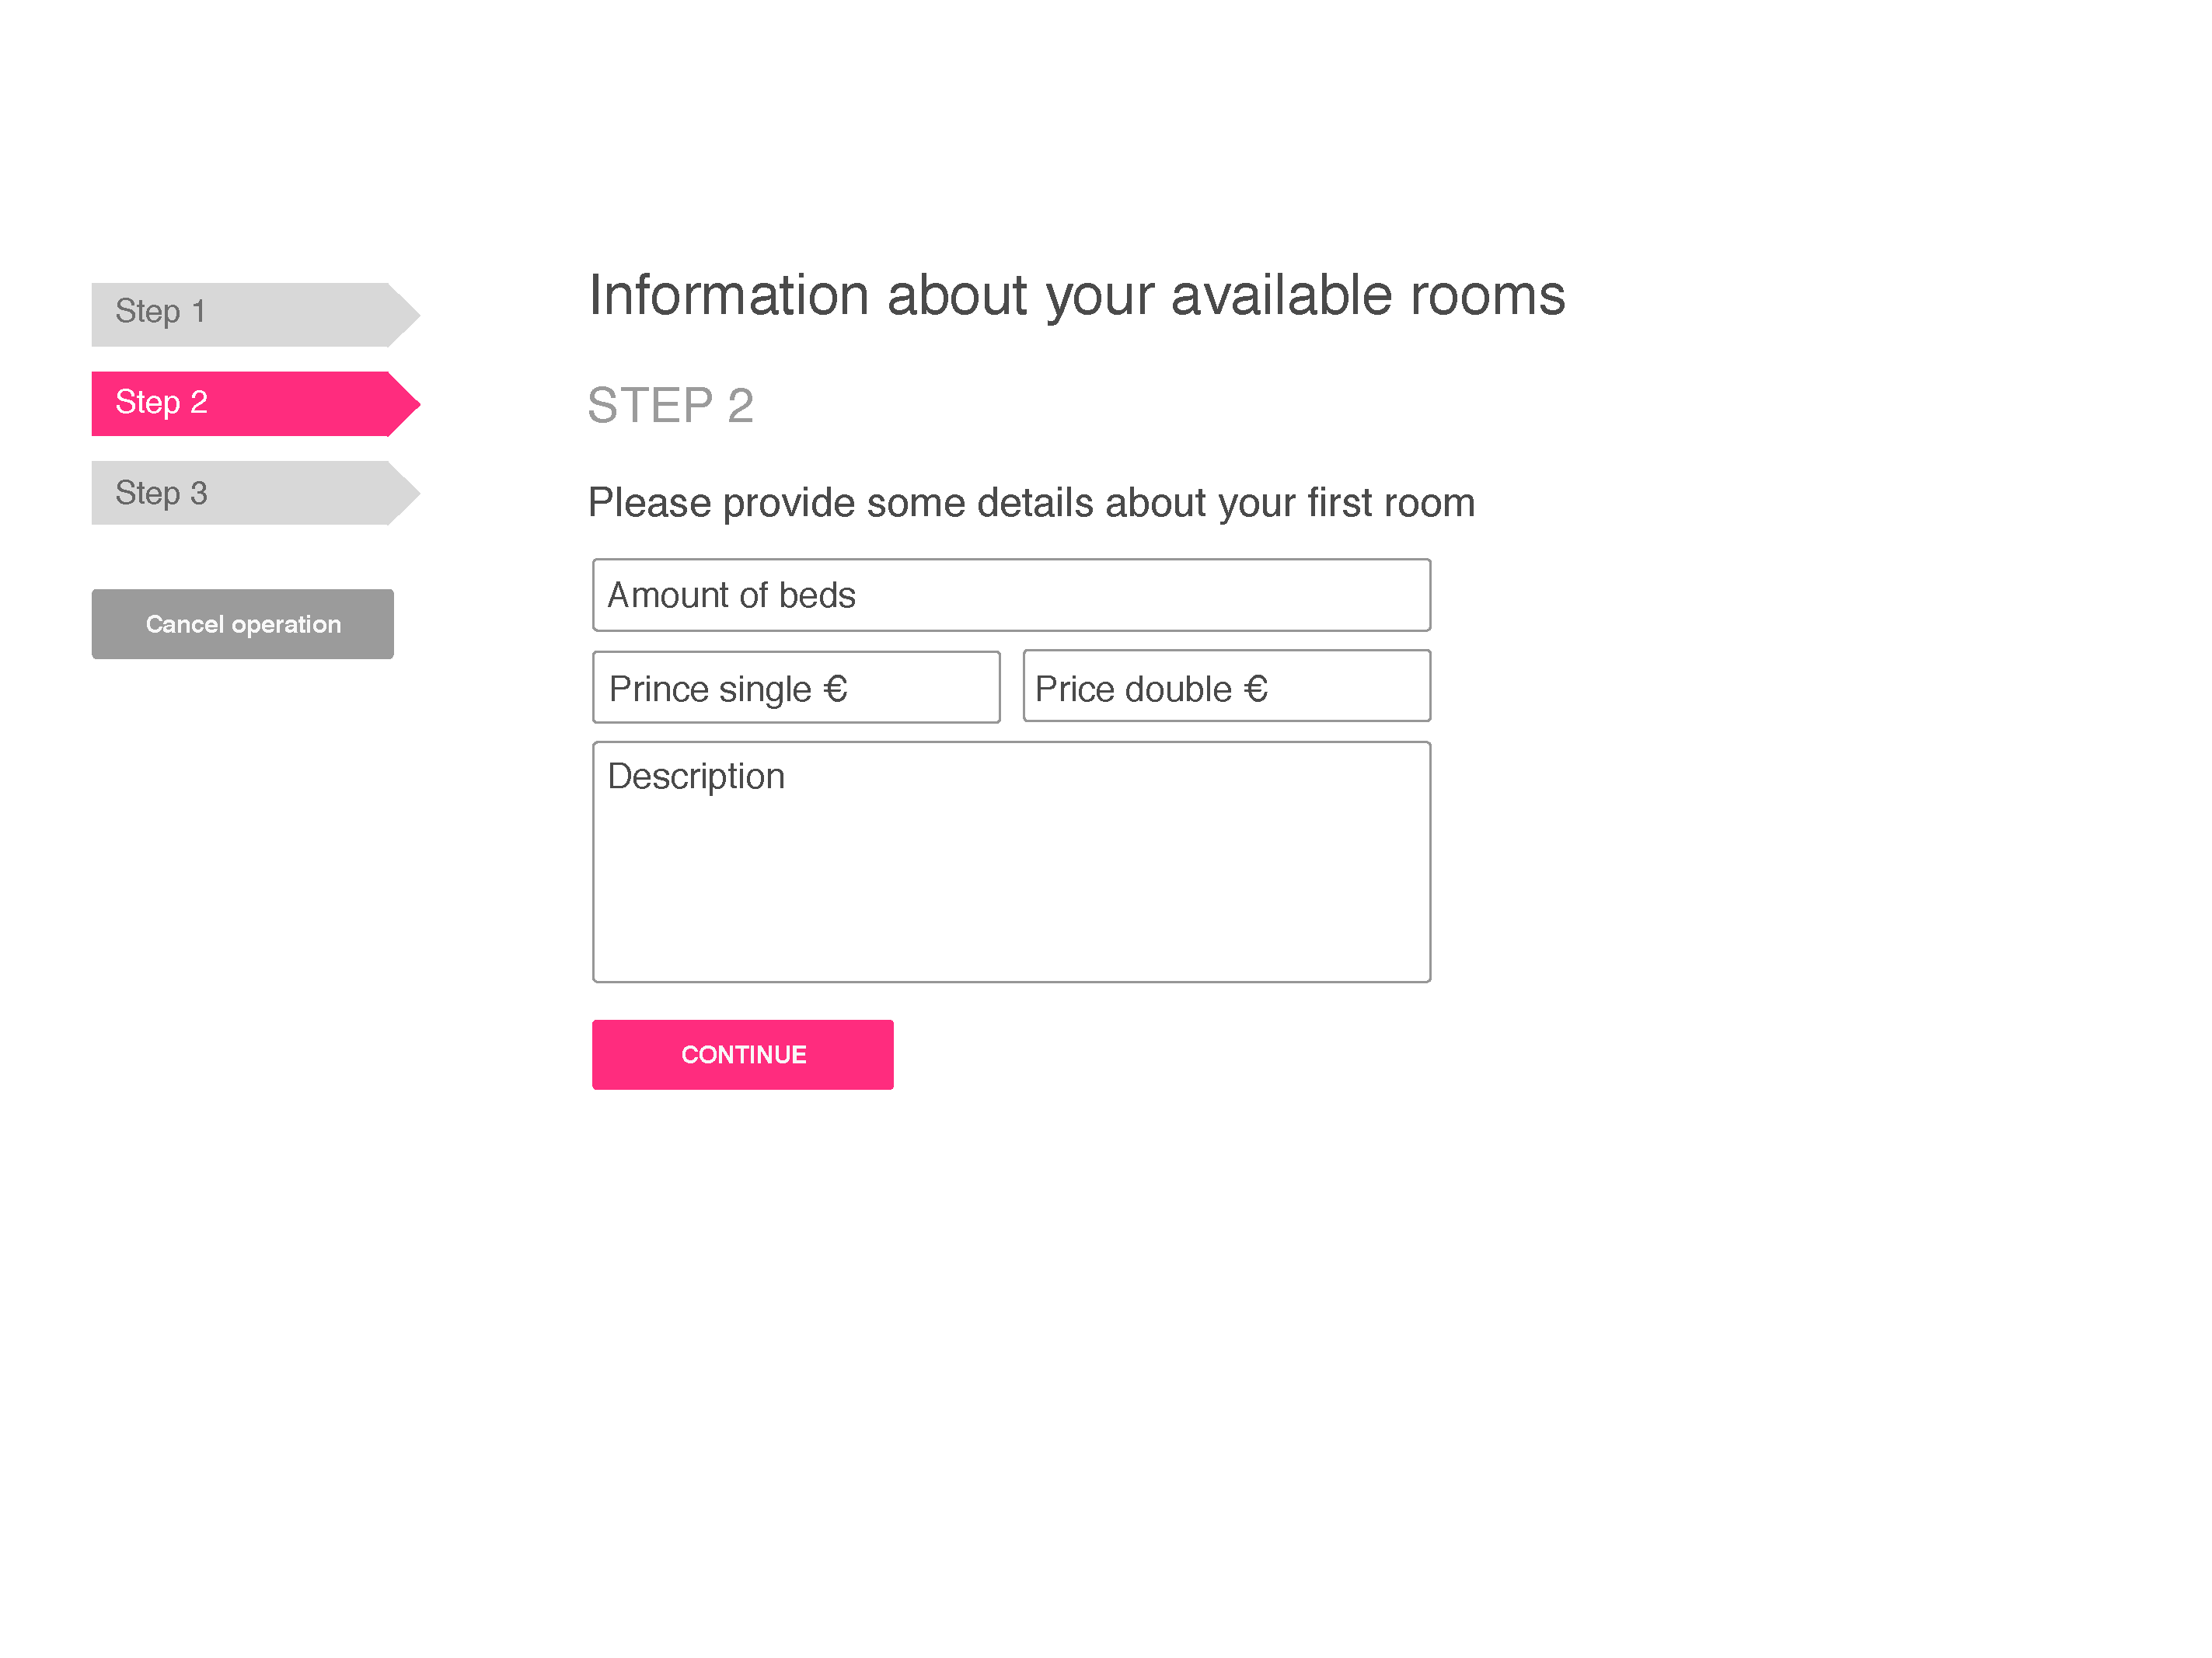
\includegraphics[width=\textwidth]{img/mockups/host_registerproperty2.pdf}
      \caption{Register a property (2/3)}
      \label{register_a_property2}
    \end{minipage}

    \\

    \begin{minipage}[b]{0.5\textwidth}
      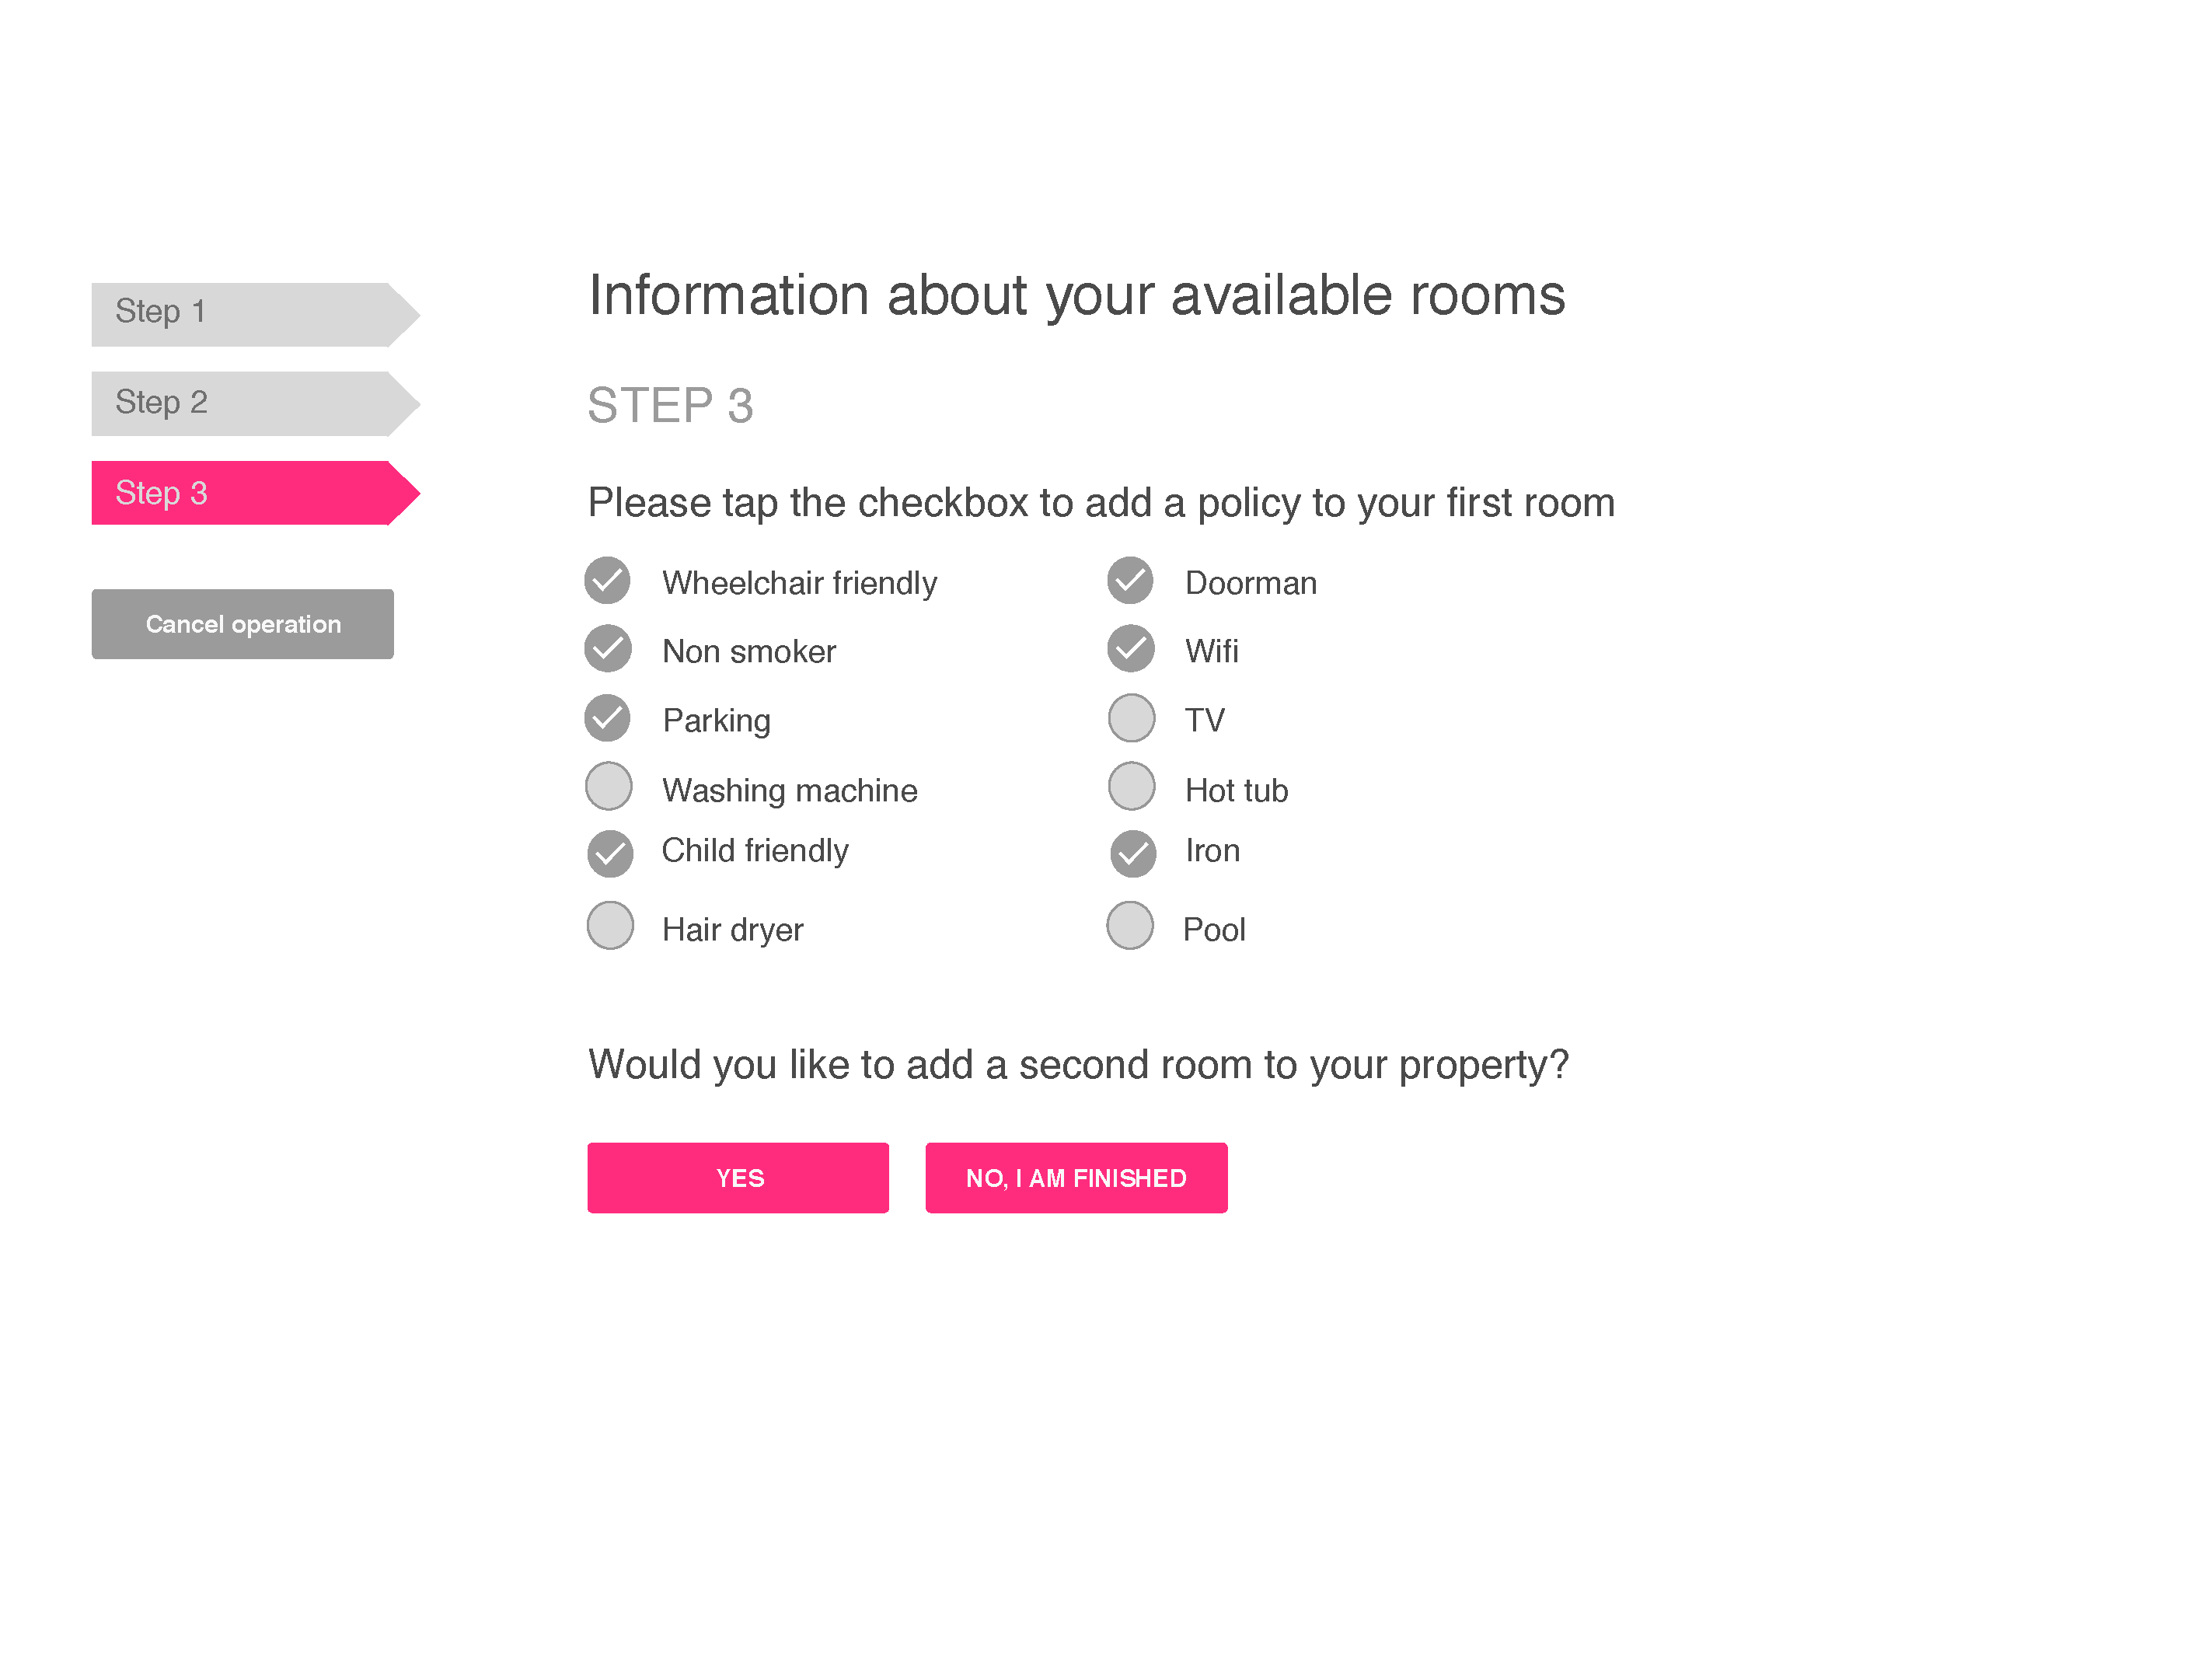
\includegraphics[width=\textwidth]{img/mockups/host_registerproperty3.pdf}
      \caption{Register a property (3/3)}
      \label{register_a_property3}
    \end{minipage}
    \begin{minipage}[b]{0.5\textwidth}
      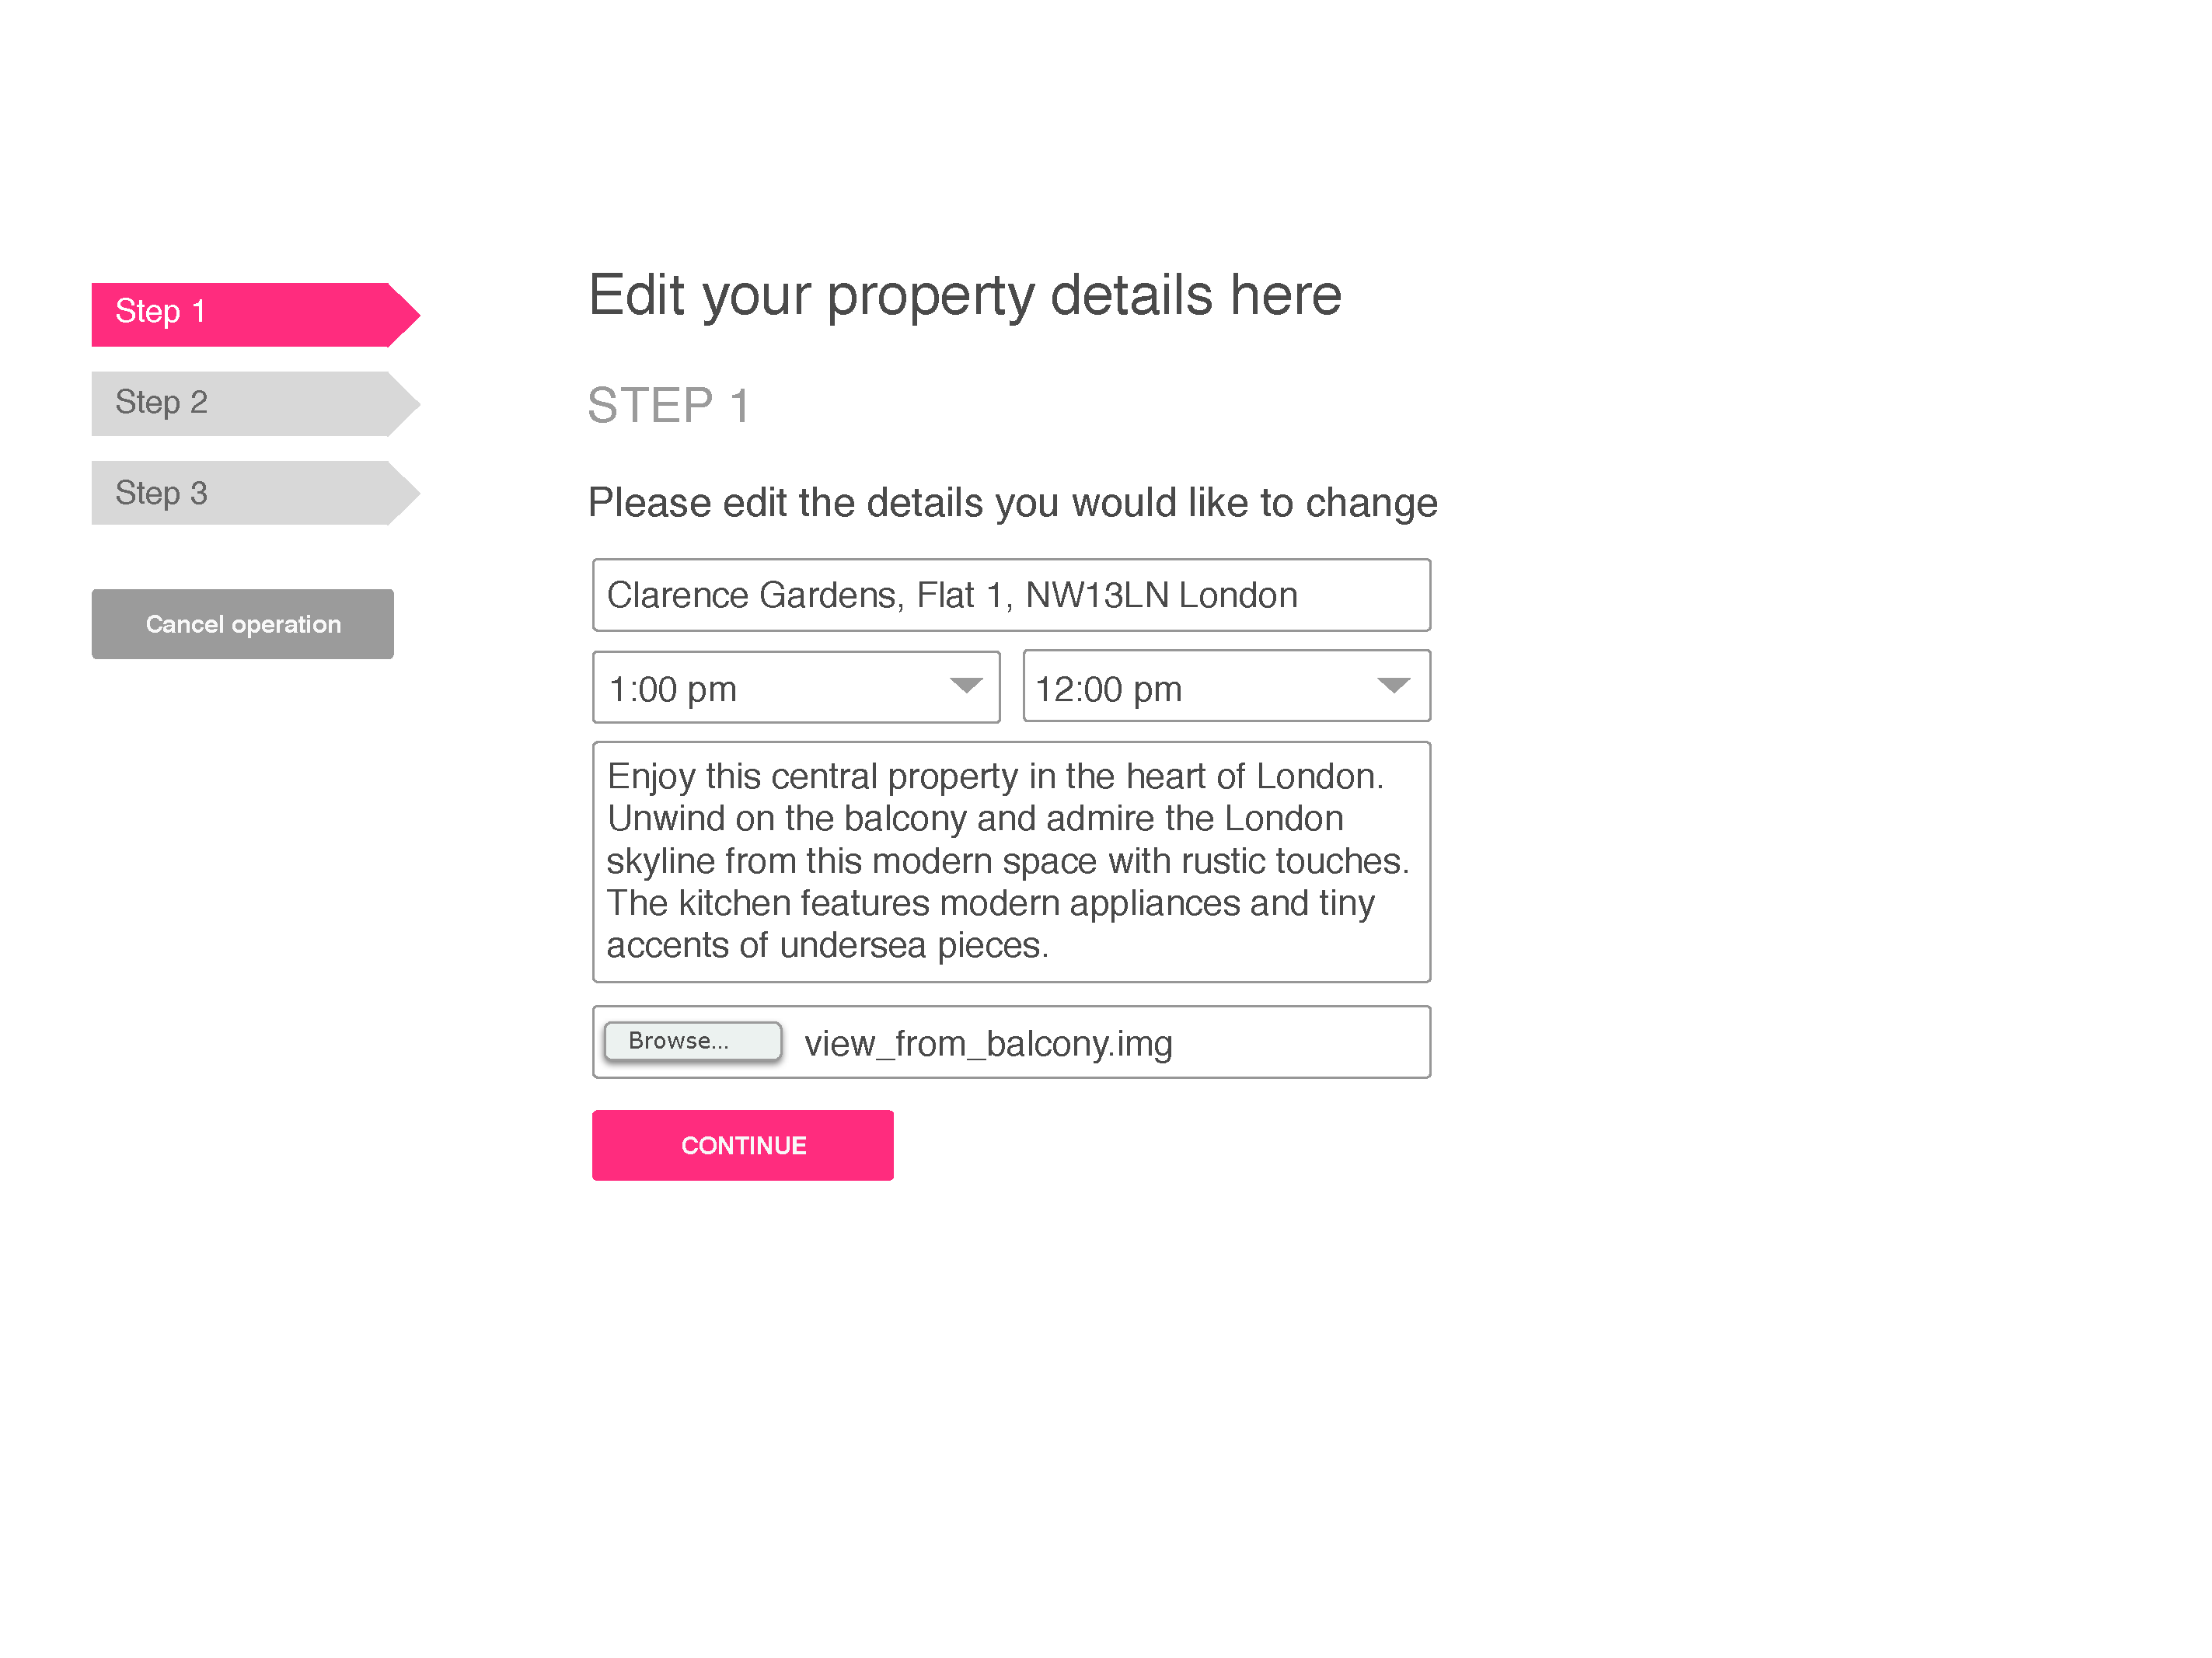
\includegraphics[width=\textwidth]{img/mockups/host_editproperty1.pdf}
      \caption{Edit a property (1/3)}
      \label{edit_a_property1}
    \end{minipage}

    \\

    \begin{minipage}[b]{0.5\textwidth}
      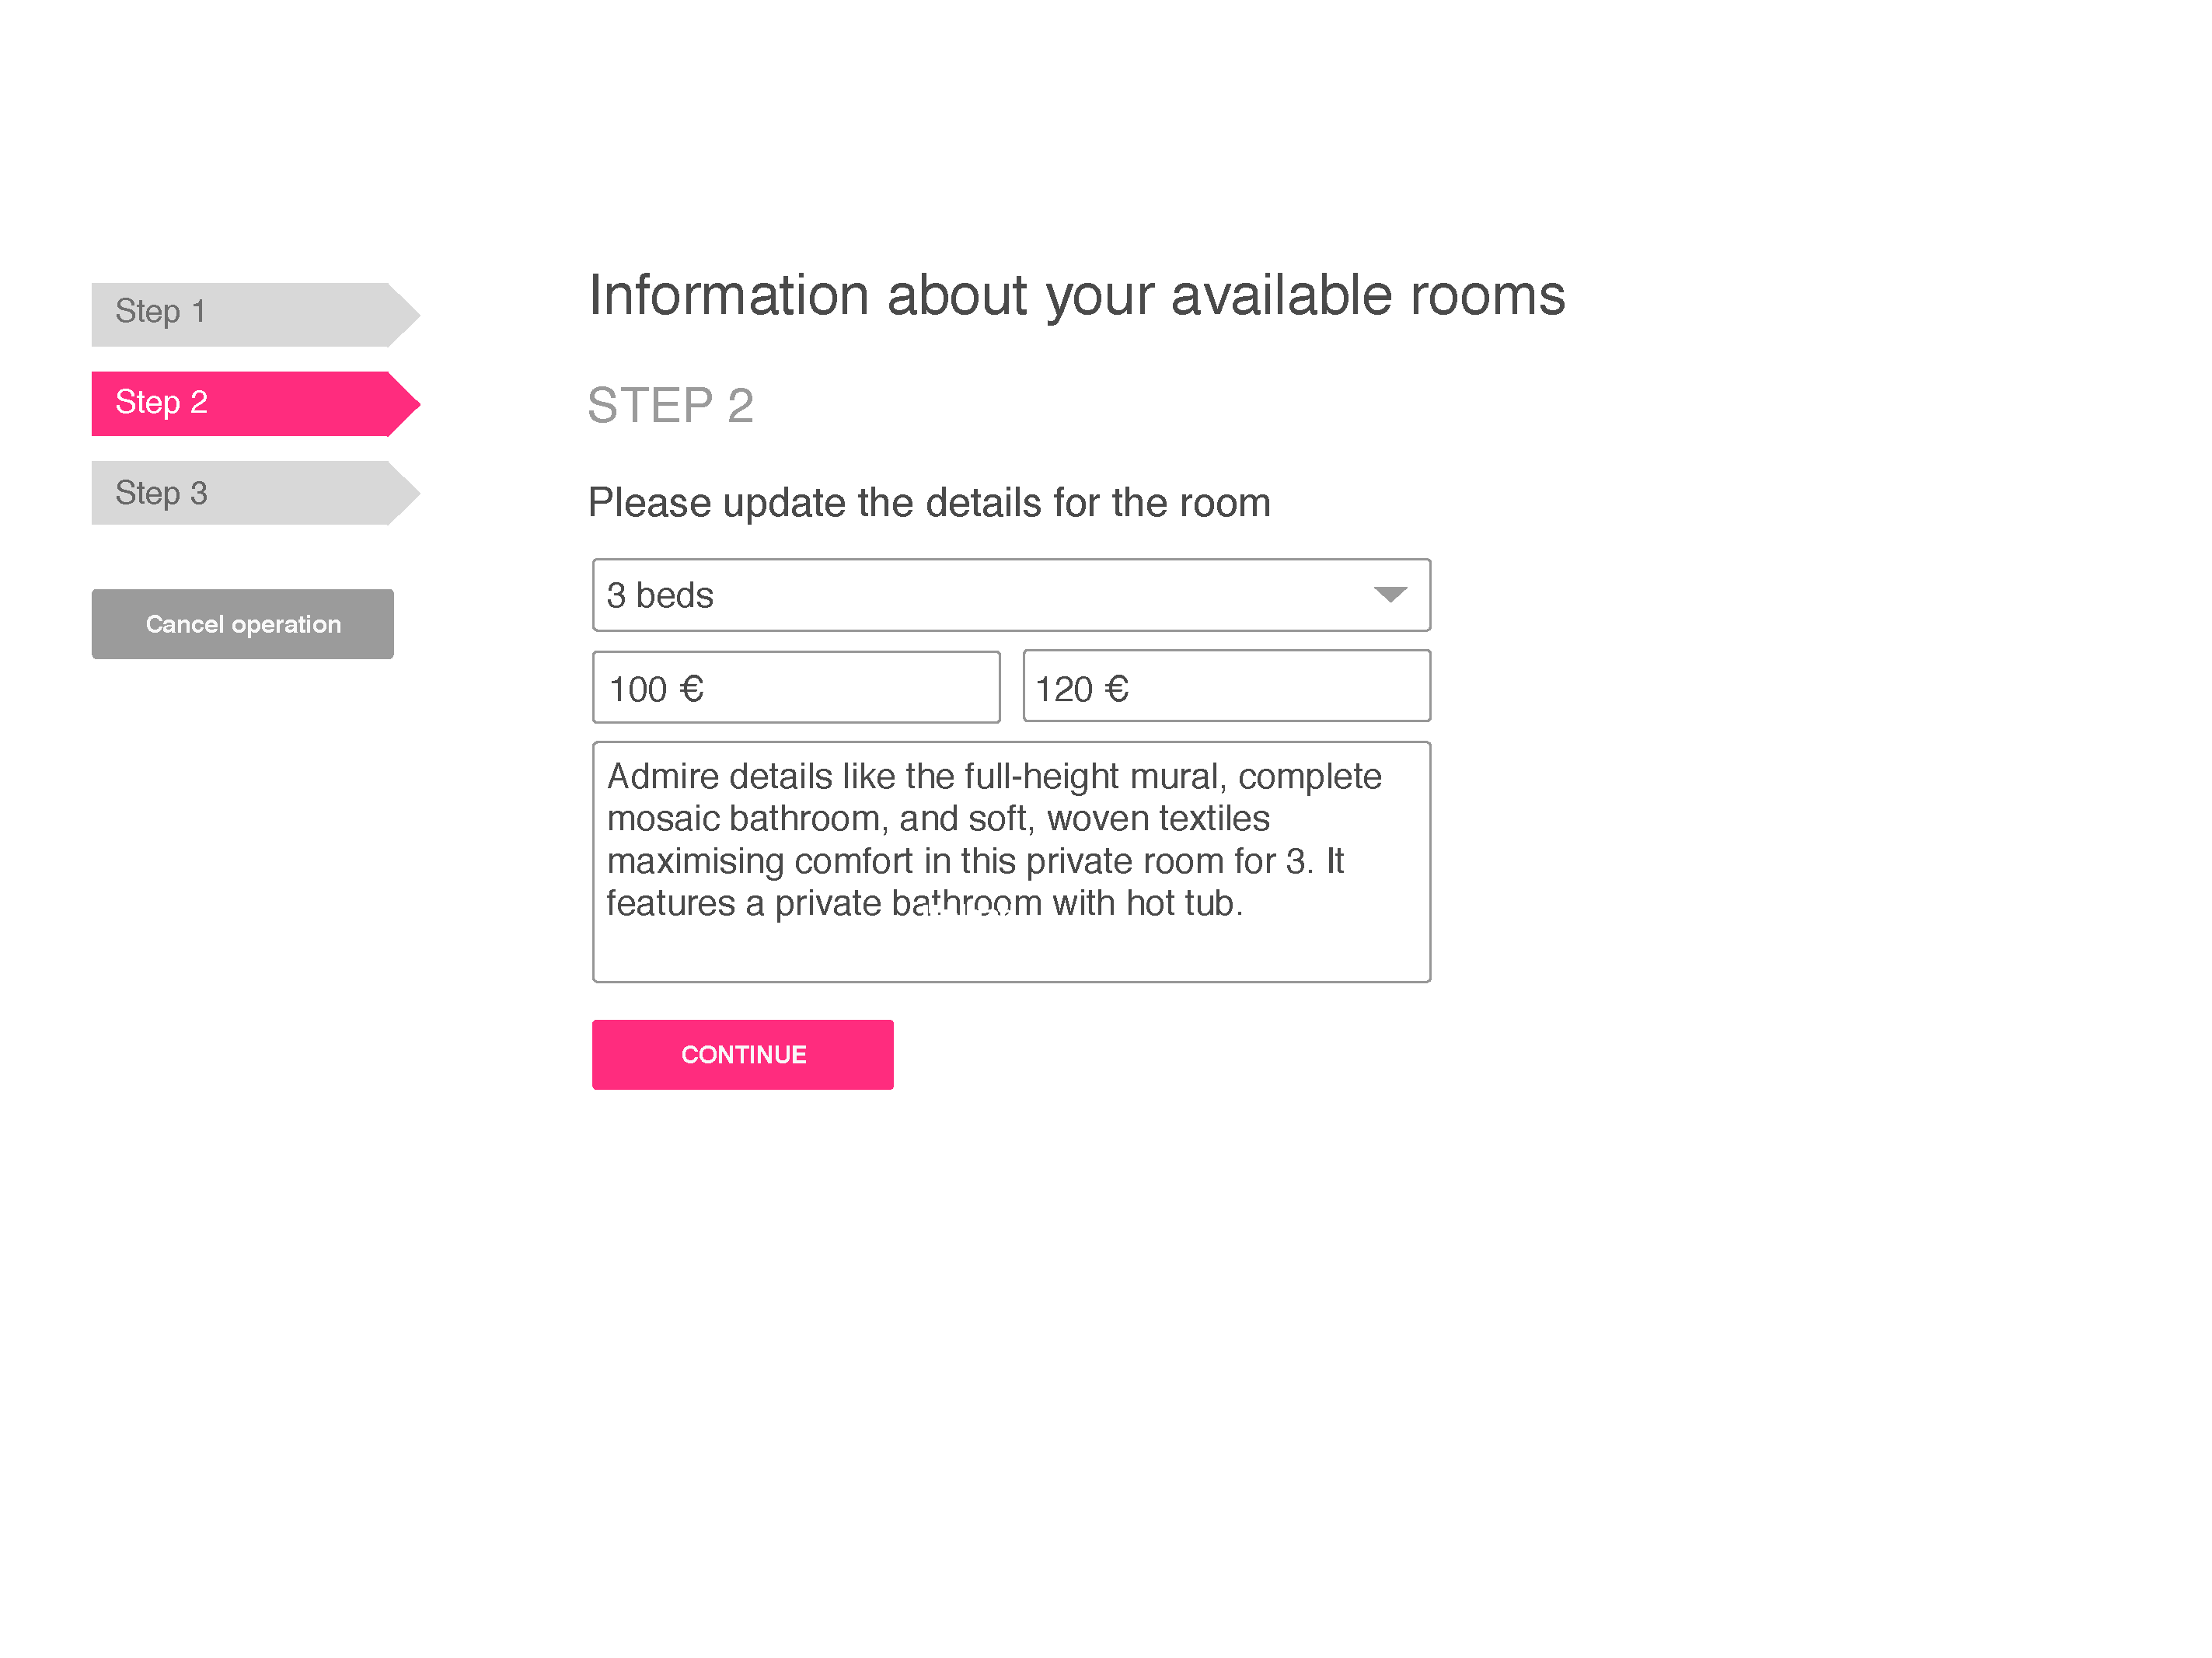
\includegraphics[width=\textwidth]{img/mockups/host_editproperty2.pdf}
      \caption{Edit a property (2/3)}
      \label{edit_a_property2}
    \end{minipage}
    \begin{minipage}[b]{0.5\textwidth}
      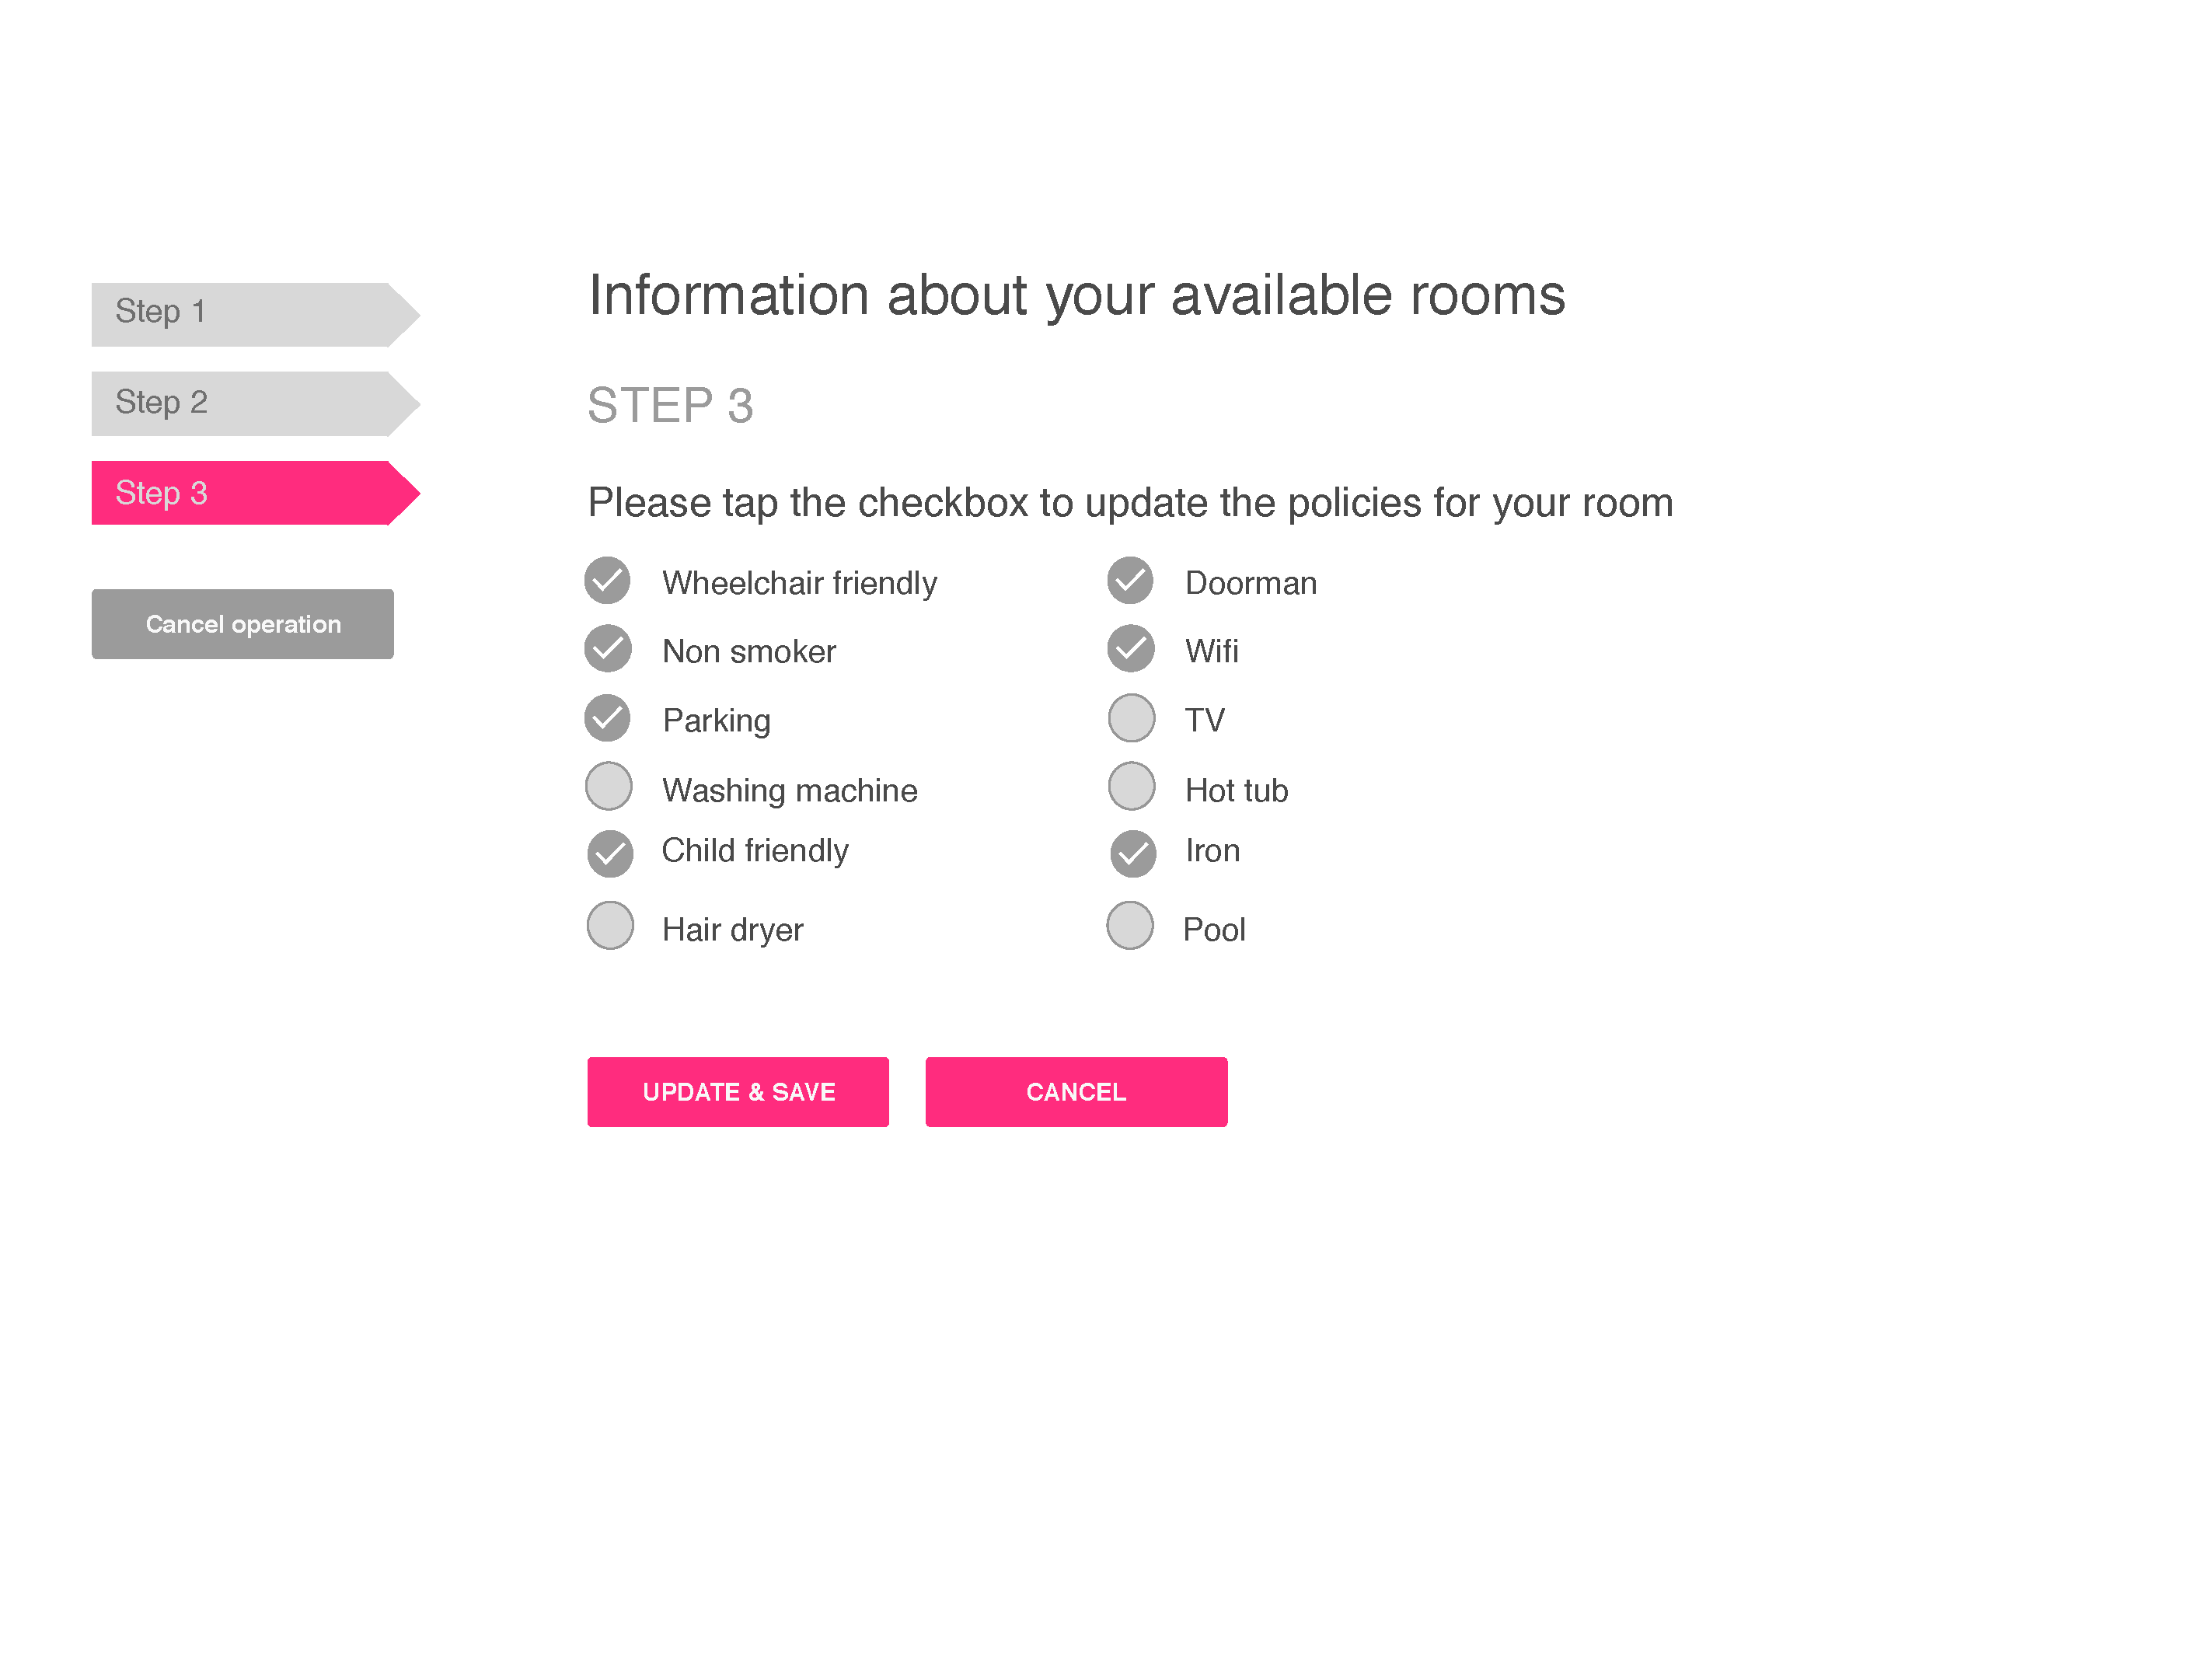
\includegraphics[width=\textwidth]{img/mockups/host_editproperty3.pdf}
      \caption{Edit a property (3/3)}
      \label{edit_a_property3}
    \end{minipage}
  \end{tabular}
\end{figure}

\section{Admin Views}
\subsection{The Admin's User Dashboard} \label{admindashboard_section}
The Admin has three main responsibilities: managing the Users of the platform, creating the Policies for the rooms, and overseeing the Properties. After logging in, the Admin lands on a dashboard where a list of all platform Users is depicted. Here, they have the option to edit/add a user. A User is added through a simple popup view that appears when issuing the request to create one. After submitting the required information and indicating the new User's Role, the new User receives an email to confirm their details.

When requesting to edit a User's personal details on the dashboard, the Admin can view the User's information and edit everything except for the email and password. The password is not visible. The Admin's information also appears on this list, enabling the Admin to edit their own personal details in this view as well.

A menu on the left side leads the Admin to the policy list or to the same search view the Guest sees when clicking on "Manage properties".

\begin{figure}[H]
  \centering
  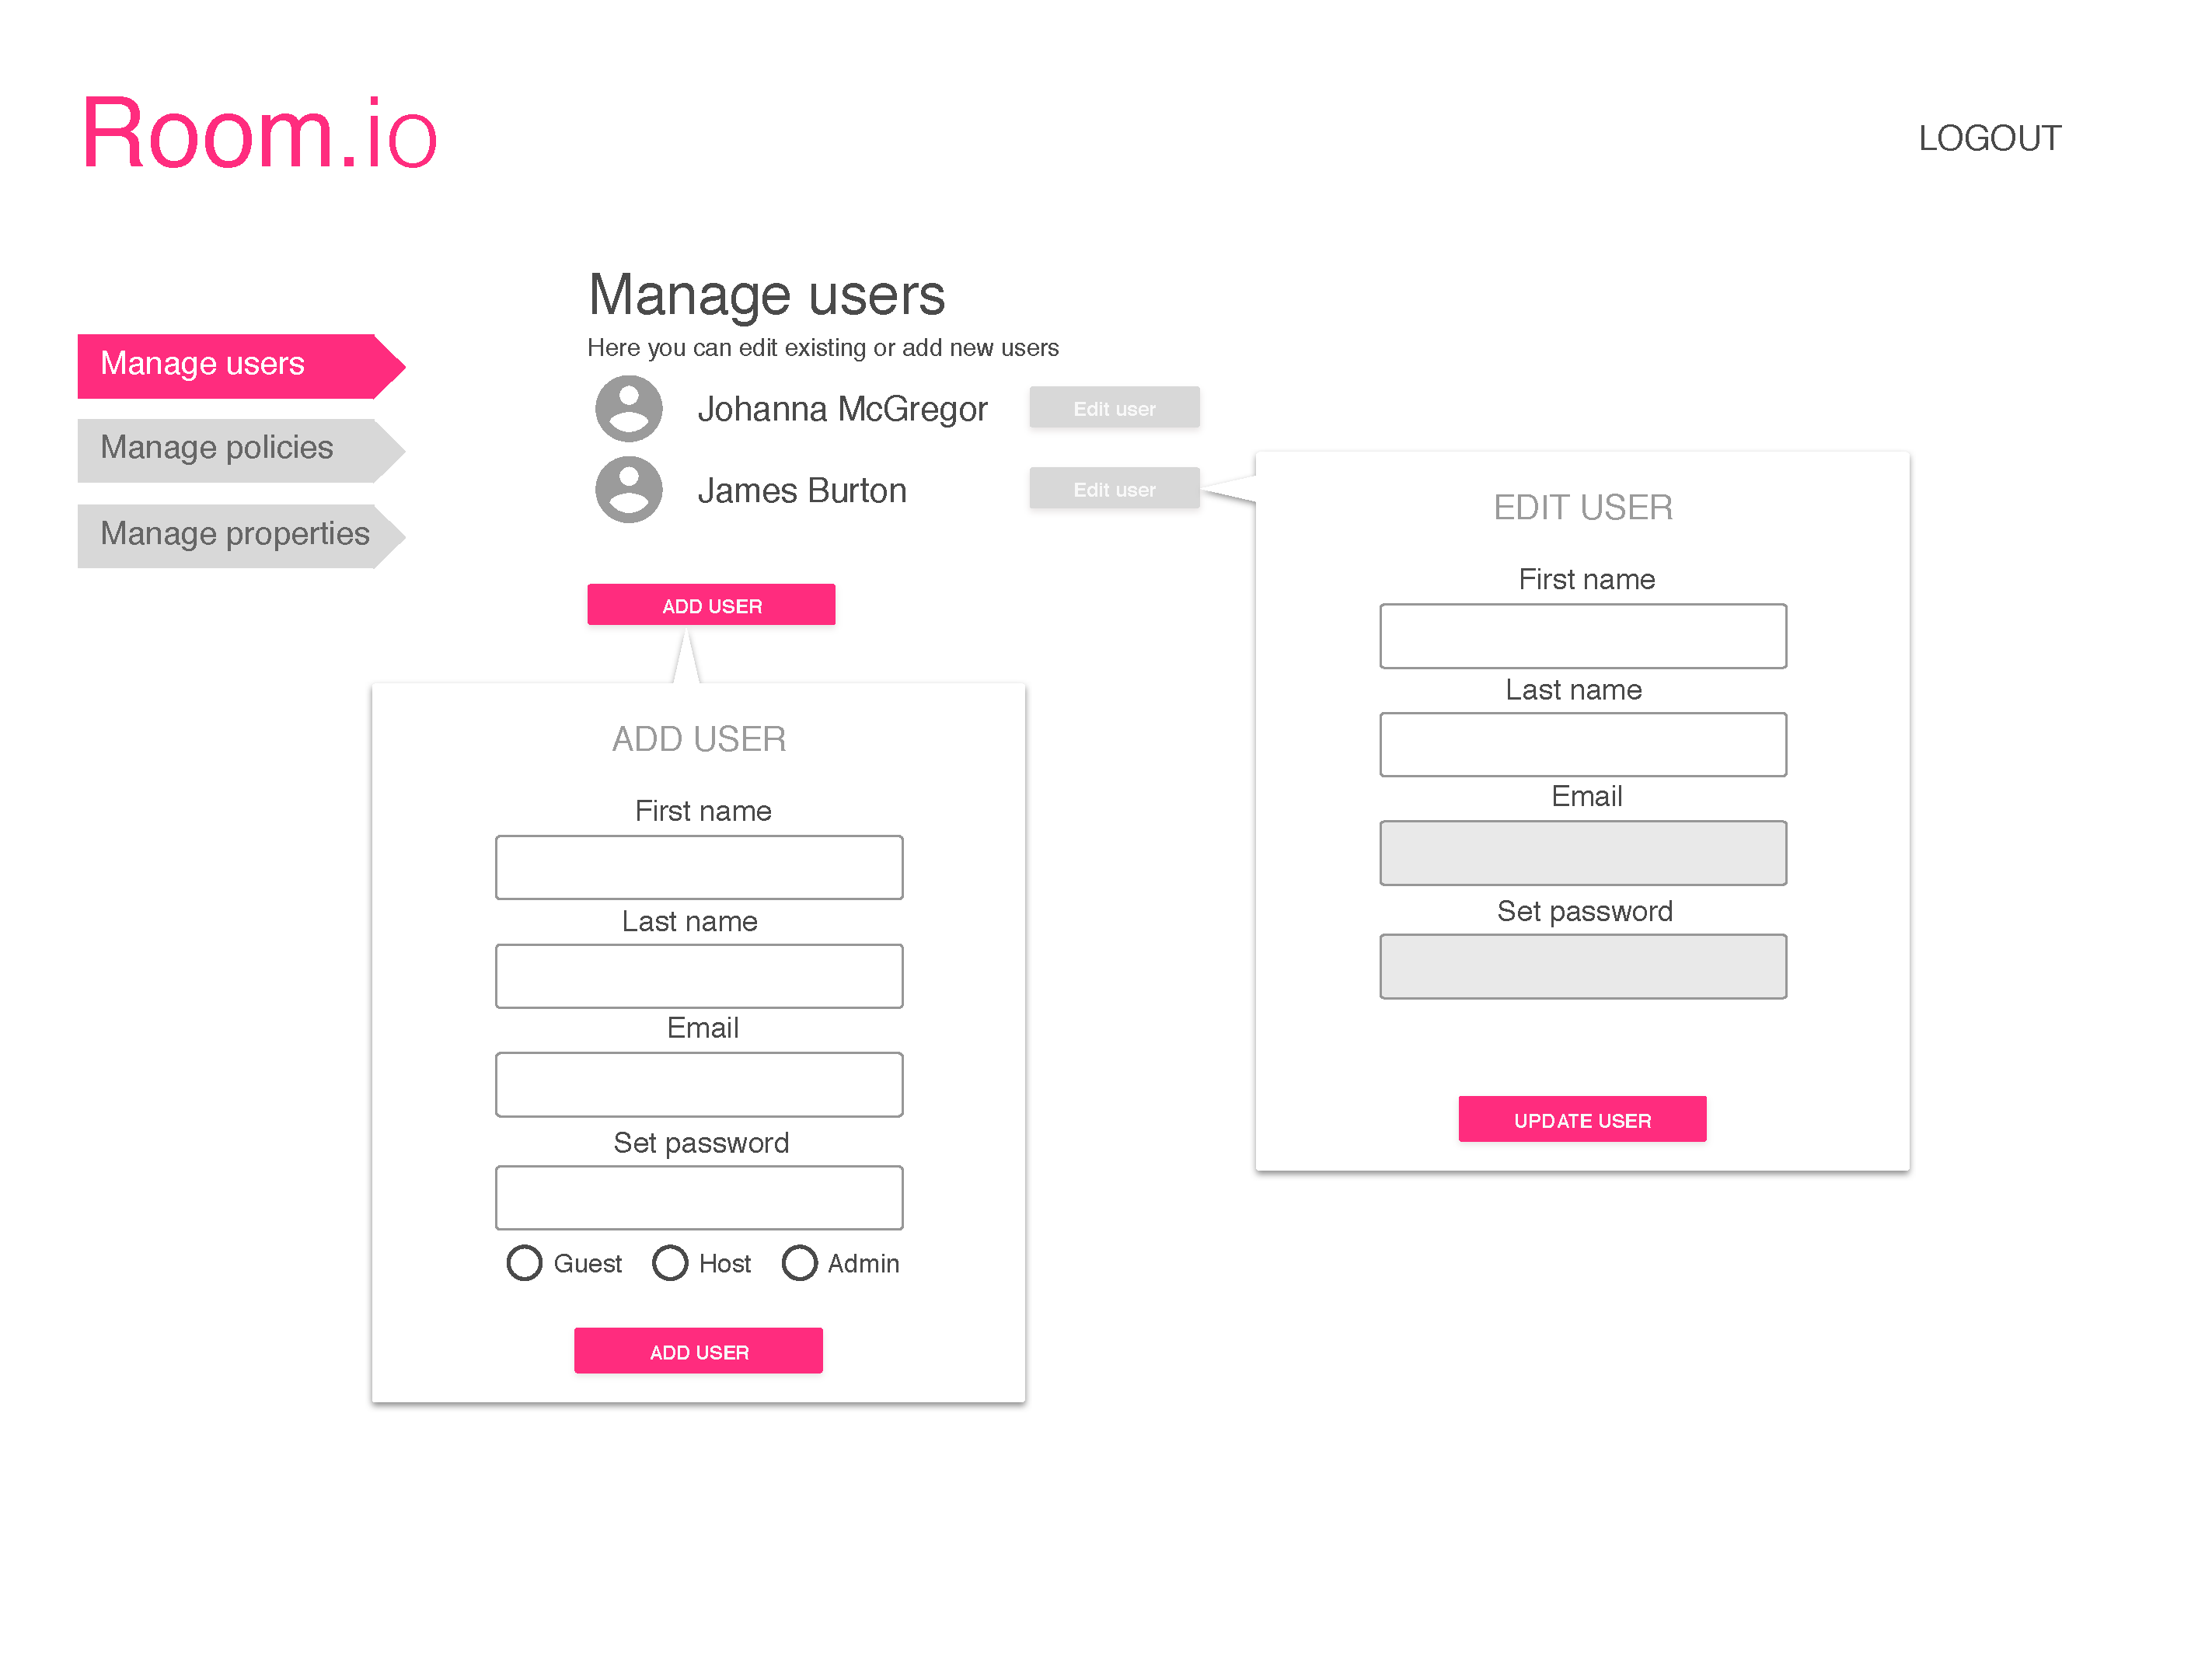
\includegraphics[width=\textwidth]{img/mockups/admin_dashboard.pdf}
  \caption{Admin dashboard}
  \label{admin_dashboard}
\end{figure}

\subsection{Policy list}
The Admin is responsible for creating and editing a list of policies for rooms that can be selected by the Hosts when creating a property. Room policies can include house rules such as "no smoking" in addition to amenities and room properties such as "wheelchair friendly" and "concierge". On this page, the Admin has the possibility to delete or add new Policies to the list.

\begin{figure}[H]
  \centering
  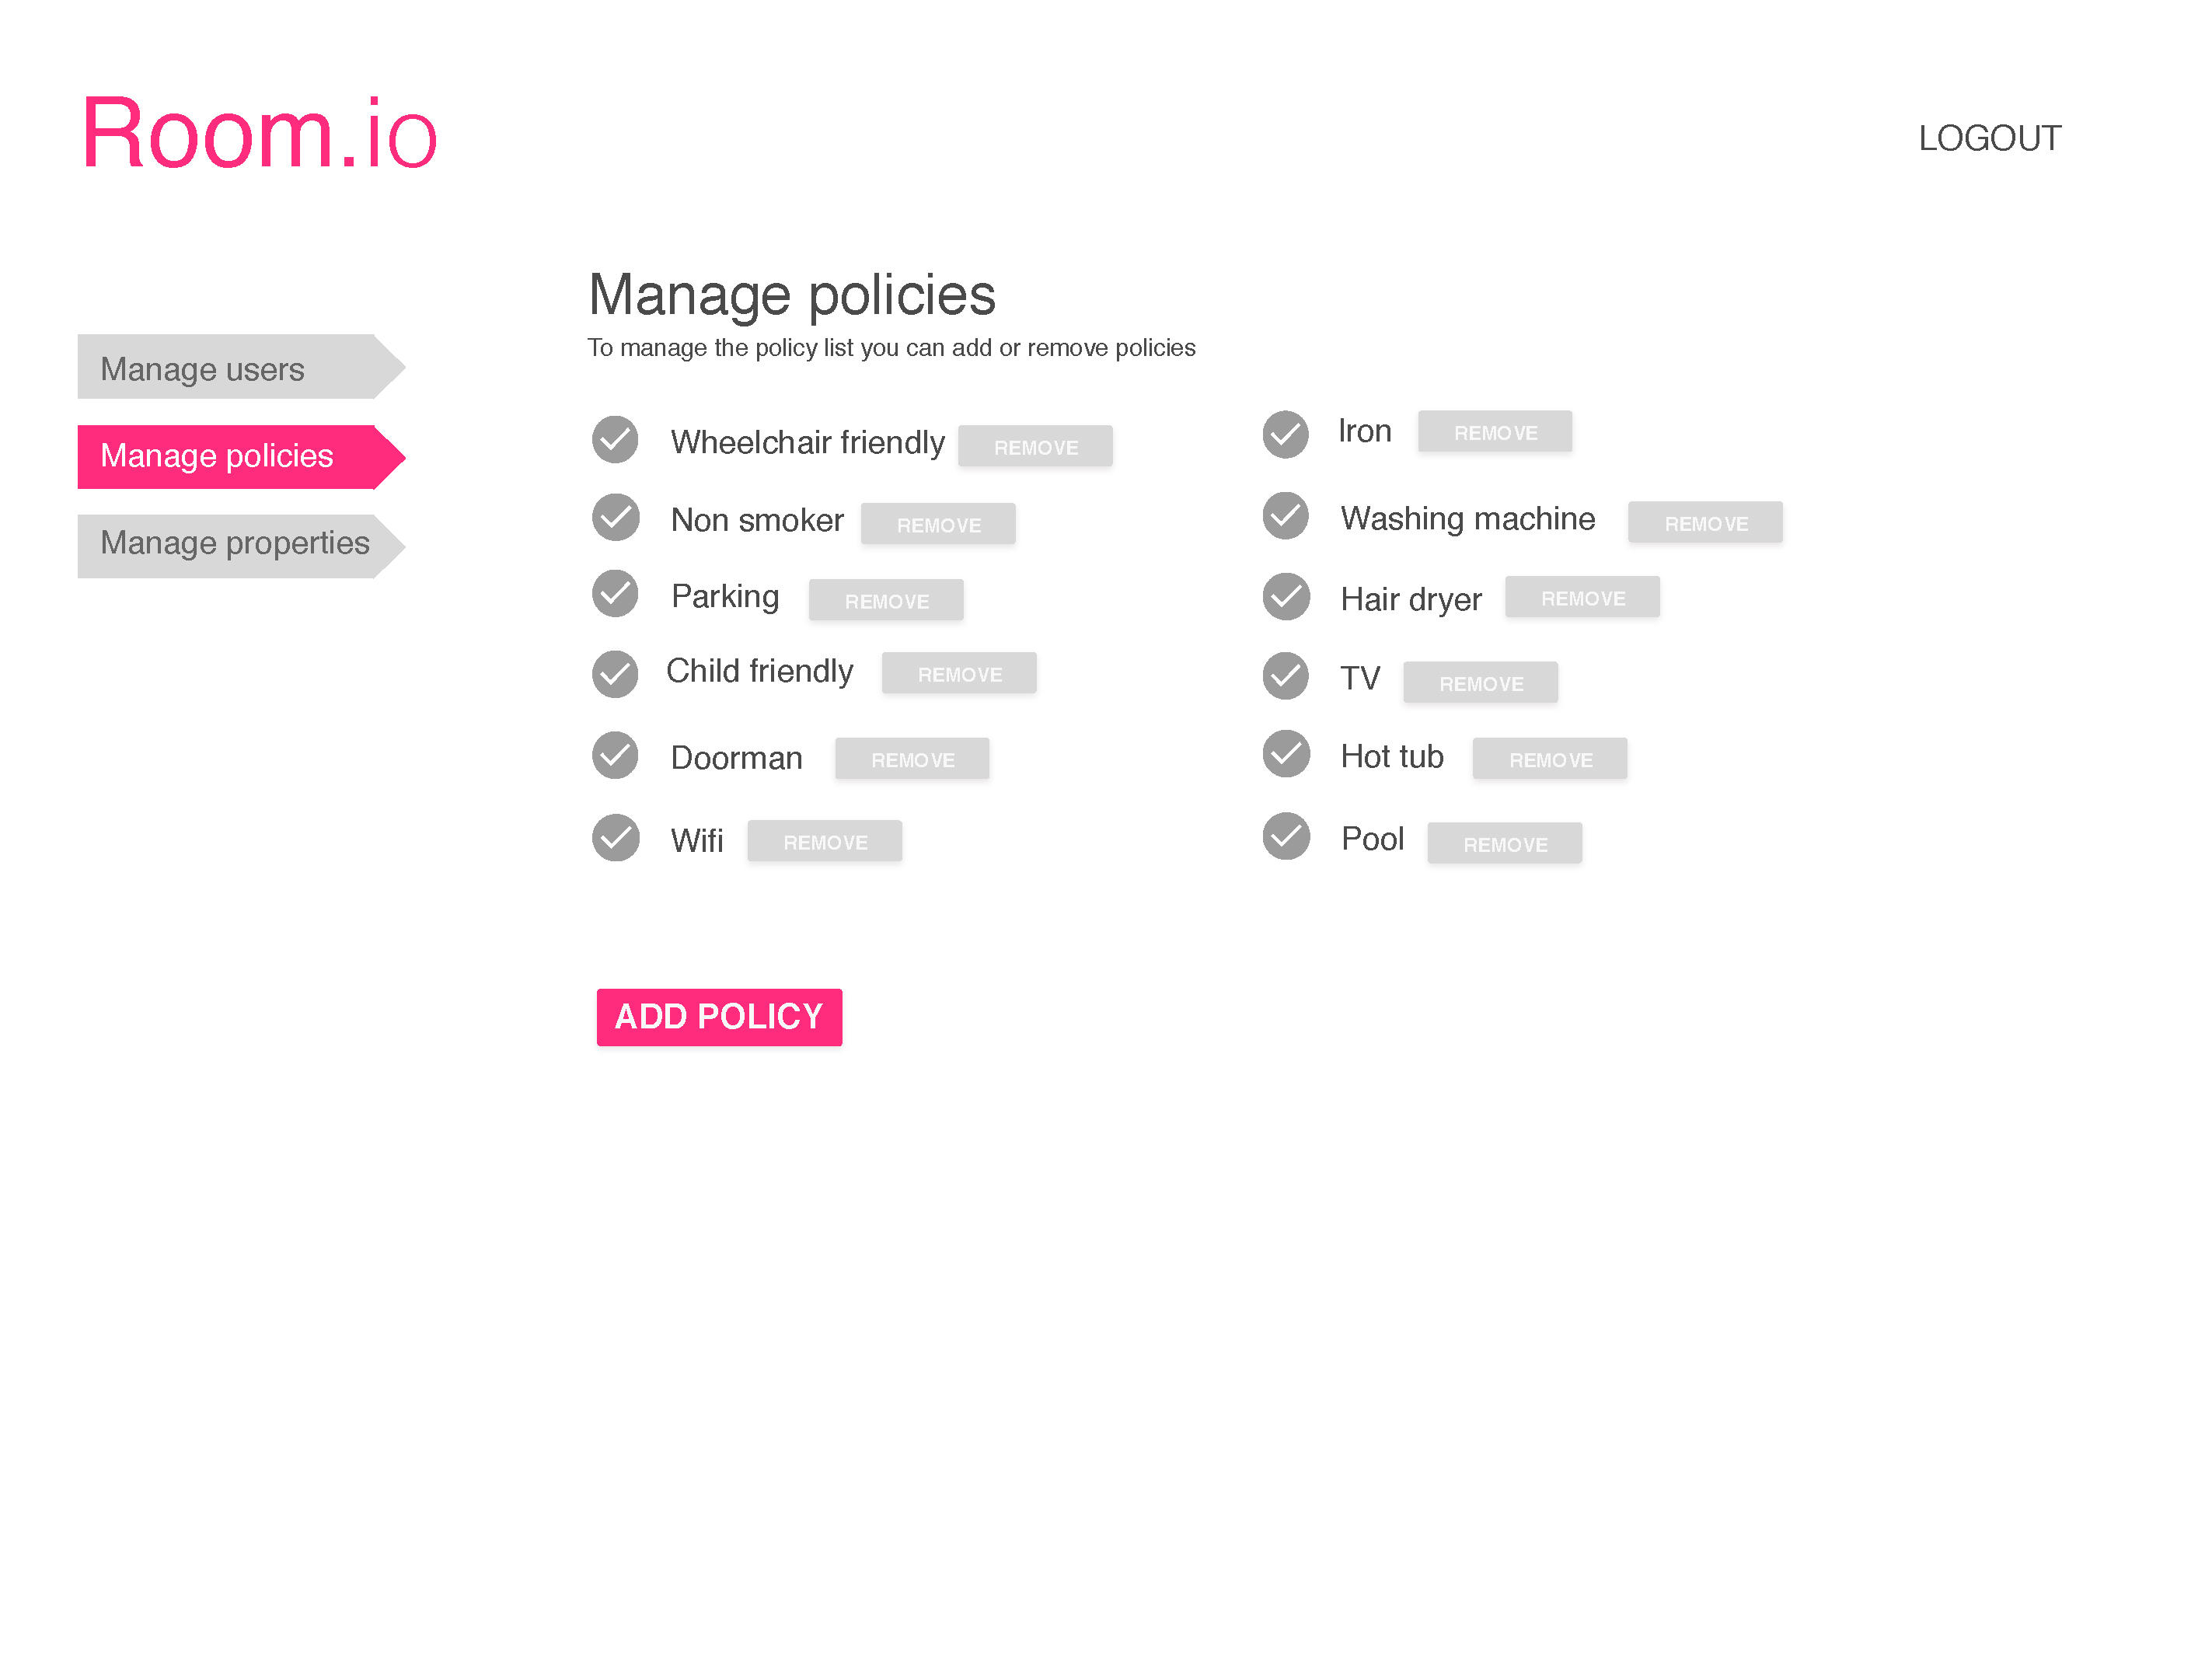
\includegraphics[width=\textwidth]{img/mockups/admin_policies.pdf}
  \caption{Policy list}
  \label{admin_policy}
\end{figure}
